\section{Side projects}

\subsection{Cosmological SIMS}
\textbf{Using the Gadget-2 code, two cosmological simulations with $128^3$ and $256^3$ dark matter particles were run in a cosmological box with a co-moving volume of (10 Mpc$)^3$. Gravitational softenings of 7.4 and 1.8 kpc were used, respectively. The simulations were initiated at $z=63$, and the initial conditions were created with the public N-GenIC code, available at the Gadget website: 
\url{http://www.mpa-garching.mpg.de/gadget/}} \\ \\


\subsection{Velocity distribution functions}
\begin{figure}
\centering
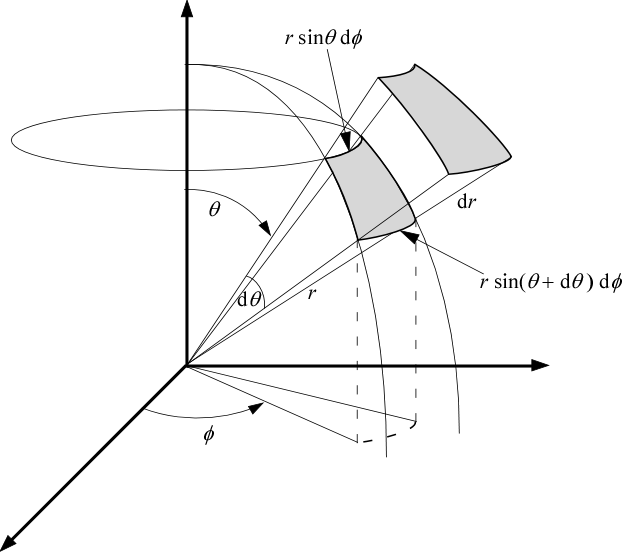
\includegraphics[width=1.0 cm]{img/control-volume-spherical.png}
\caption{Spherical coordinates $ r, \theta $ and $ \phi$. The 3 boldtype coordinate axes represent the Cartesian axes x, y and z. The grey areas shows two small surface areas of concentric spheres around Origo, which together define a small volume element in configuration space. With $ r \geq 0 $, $ \theta \in [0 ; \pi] $ and $ \phi \in [0 ; 2\pi] $ we can define any point in space. credit: http://pleasemakeanote.blogspot.dk/2010/02/9-derivation-of-continuity-equation-in.html}
\label{fig:test}
\end{figure}

Velocity distribution functions (VDF's) are fundamentally important in order to understand the behavior of DM dynamics.

The initial velocity distributions are Gaussian and have velocity dispersions,  $ \sigma_{rad}$  and $\sigma_{tan} $, which I later use in the analysis code (they can be found from the Jeans equation, see previous section). It is worth mentioning that in reality, the velocity distributions is probably not Gaussian but the velocity is anisotropic. The Dark Matter velocity is badly understood, however this will normally not effect the discovery of dark matter in direct experiments. But it is critically important to understand the DM velocity better in order to compare different experiments with each other, as well as comparing direct detections with colliders. So it is crucial to develop a better understanding in order to detect the actual DM particles. 


The total velocity of each particle is decomposed into the 1D radial velocity, and the 2D tangential velocity which can be further decomposed into 
two mutually orthogonal velocity vectors residing in the tangential plane of the halo wrt the radius vector. They are $v_{\theta}$ and $v_{\phi}$.

From the cartesian coordinates, the spherical coordinates can be found: \\
\begin{equation}
\begin{aligned}
&r = \sqrt{x^2+y^2+z^2} \\ 
&\theta = arccos \bigg(\frac{z}{|\boldsymbol{r}|} \bigg)  \\
& \phi = arctan \bigg(\frac{y}{x} \bigg) \\
\end{aligned}
\end{equation}

Similarly,
\begin{equation}
\begin{aligned}
&x = \boldsymbol{r} sin\theta cos\phi \\ 
&y = \boldsymbol{r} sin\theta sin\phi  \\
&z = \boldsymbol{r} cos\theta \\
\end{aligned}
\end{equation}

The total velocity vector can be expressed in terms of Cartesian unit vectors, $\hat{i} , \hat{j}$ and $\hat{k}$, as 
\begin{equation}
     \boldsymbol{v}=\begin{bmatrix}
         v_x \\
         v_y \\
         v_z\\
        \end{bmatrix}
        = v_x\hat{i}+v_y\hat{j}+v_z\hat{k}
\end{equation}
Or wrt the spherical unit vectors , $\hat{r} , \hat{\theta}$ and $\hat{\phi}$, as 
\begin{equation}
     \boldsymbol{v}=\begin{bmatrix}
         \dot{r} \\
         r\dot{\theta} \\
         r\dot{\phi}sin\theta \\
        \end{bmatrix}
        = \dot{r}\hat{r}+r\dot{\theta}\hat{\theta}+r\dot{\phi}sin\theta\hat{\phi}
\end{equation}
So the radial velocity becomes
\begin{equation}
\begin{aligned}
\boldsymbol{v_r} &= \frac{\boldsymbol{r}\cdot \boldsymbol{v}}{|\boldsymbol{r}|} = \frac{x\cdot v_x + y\cdot v_y + z\cdot v_z}{|\boldsymbol{r}|} =\\
& \frac{|\boldsymbol{r}| \cdot sin\theta cos\phi \cdot v_x + |\boldsymbol{r}| \cdot sin\theta sin\phi \cdot v_y + |\boldsymbol{r}| \cdot cos\theta  \cdot v_z + }{|\boldsymbol{r}|} =\\
& sin(\theta)cos(\phi)v_x + sin(\theta)sin(\phi)v_y+ cos(\theta)v_z  \\
\end{aligned}
\end{equation}
the tangential velocity component $ v_{\theta}$ is
\begin{equation}
\begin{aligned}
\boldsymbol{v_{\theta}} &= 
\frac{\frac{d\boldsymbol{r}}{d\theta} \cdot \boldsymbol{v}}{|\boldsymbol{r}|} = \\
&\frac{\frac{d}{d\theta} \cdot (r sin\theta cos\phi)\cdot v_x + 
\frac{d}{d\theta} \cdot (r sin\theta sin\phi)\cdot v_y + 
\frac{d}{d\theta} \cdot (r cos\theta)\cdot v_z}{|\boldsymbol{r}|} = \\
&cos(\theta)cos(\phi)v_x + cos(\theta)sin(\phi)v_y + sin(\theta)v_z  \\
\end{aligned}
\end{equation}
the tangential velocity component $ v_{\phi}$ is
\begin{equation}
\begin{aligned}
\boldsymbol{v_{\phi}} &= 
\frac{\frac{d\boldsymbol{r}}{d\phi} \cdot \boldsymbol{v}}{|\boldsymbol{r}|} = \\
& \frac{\frac{d}{d\phi} \cdot (r sin\theta cos\phi)\cdot v_x + 
\frac{d}{d\phi} \cdot (r sin\theta sin\phi)\cdot v_y + 
\frac{d}{d\phi} \cdot (z)\cdot v_z}{|\boldsymbol{r}|} = \\
& \frac{d}{d\phi} \cdot (cos\phi) \cdot v_x + 
\frac{d}{d\phi} \cdot (sin\phi)\cdot v_y + 0 = \\
& -sin(\phi)v_x + cos(\phi)v_y  \\
\end{aligned}
\end{equation},
since for the $\phi$-plane, $z = 0$, $\theta = 90 \deg $ and so $ sin\theta = 1$.
and finally the 2D tangential speed is
\begin{equation}
|\boldsymbol{v_{tan}}| = \sqrt{v_{\theta}^2+v_{\phi}^2}  
\end{equation}
In order to better compare different radial bins, each velocity or speed is normalized by dividing them with their corresponding velocity dispersions. These new dimensionless normalized velocities and speeds are denoted by u;
The radial normalized velocity is 
\begin{equation}
\boldsymbol{u_r} = \frac{\boldsymbol{v_r}}{\sigma_r}
\end{equation}
and the tangential normalized speed is 
\begin{equation}
\boldsymbol{u_t} = \sqrt{\boldsymbol{u_{\theta}}^2+\boldsymbol{u_{\phi}}^2}  =      
\sqrt{\bigg(\frac{\boldsymbol{v_{\theta}}}{\sigma_{\theta}} \bigg)^2+\bigg(\frac{\boldsymbol{v_{\phi}}}{\sigma_{\phi}} \bigg)^2} 
\end{equation}
To see how close the VDFs are to being Gaussian, from the plots we can determine the FWHM and use the relation $ FWHM = 2 \cdot \sqrt{2 ln 2} \sigma \approx 2.355 \sigma $, where $\sigma$ is the velocity dispersion.
This value of $\sigma$ can then be compared to the real $\sigma$ that is computed directly.
The ratio $ \frac{\sigma(FWHM)}{\sigma(computed)} \cdot 100 \% $ then gives the offset in pct.

\begin{figure}
\centering
\includegraphics[width=1.0 cm]{img/o.jpeg}
\caption{A standard normal distribution, scaled appropriately for easier comparison with the following velocity histograms.}
\label{fig:test}
\end{figure}

\begin{figure}
\centering
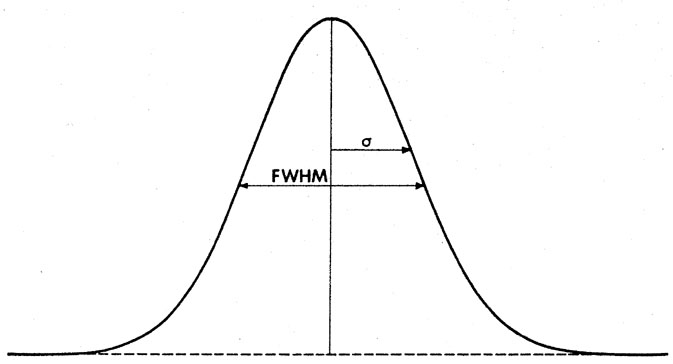
\includegraphics[width=1.0 cm]{img/figure4.jpeg}
\caption{FWHM and $\sigma$ }
\label{fig:test}
\end{figure}

A word on the dispersions: The variance of tangential velocities are defined as $\sigma_{tan}^2 = \sigma_{\theta}^2 + \sigma_{\phi}^2 $,
but this only applies when the angular momentum is the same for all directions wrt the halo centre.
That is easily checked in Python as e.g.

\begin{equation}
\begin{aligned}
L_x &= np.cross(r, v_x) \\
L_y &= np.cross(r, v_y) \\ 
L_z &= np.cross(r, v_z) \\
\end{aligned}
\end{equation}

These quantities are found to be identical.
For a spherical system of gas particles, the radial VDF would read
\begin{equation}
f(\boldsymbol{v_r}) = \exp (-\frac{\boldsymbol{v_r}^2}{2\sigma_r^2})
\end{equation}
and the tangential VDF would be
\begin{equation}
f(\boldsymbol{v_t}) = \boldsymbol{v_t} \cdot \exp (-\frac{\boldsymbol{v_t}^2}{2\sigma_t^2})
\end{equation}

The DM particle velocities is compared with two different fits: a Gaussian function $ a\cdot e^{-b\cdot x^2} $ and a more general power-law fitting function, f(q).
Figure 1 shows a comparison of a standard normal distribution function with f(q):

\begin{figure}
\centering
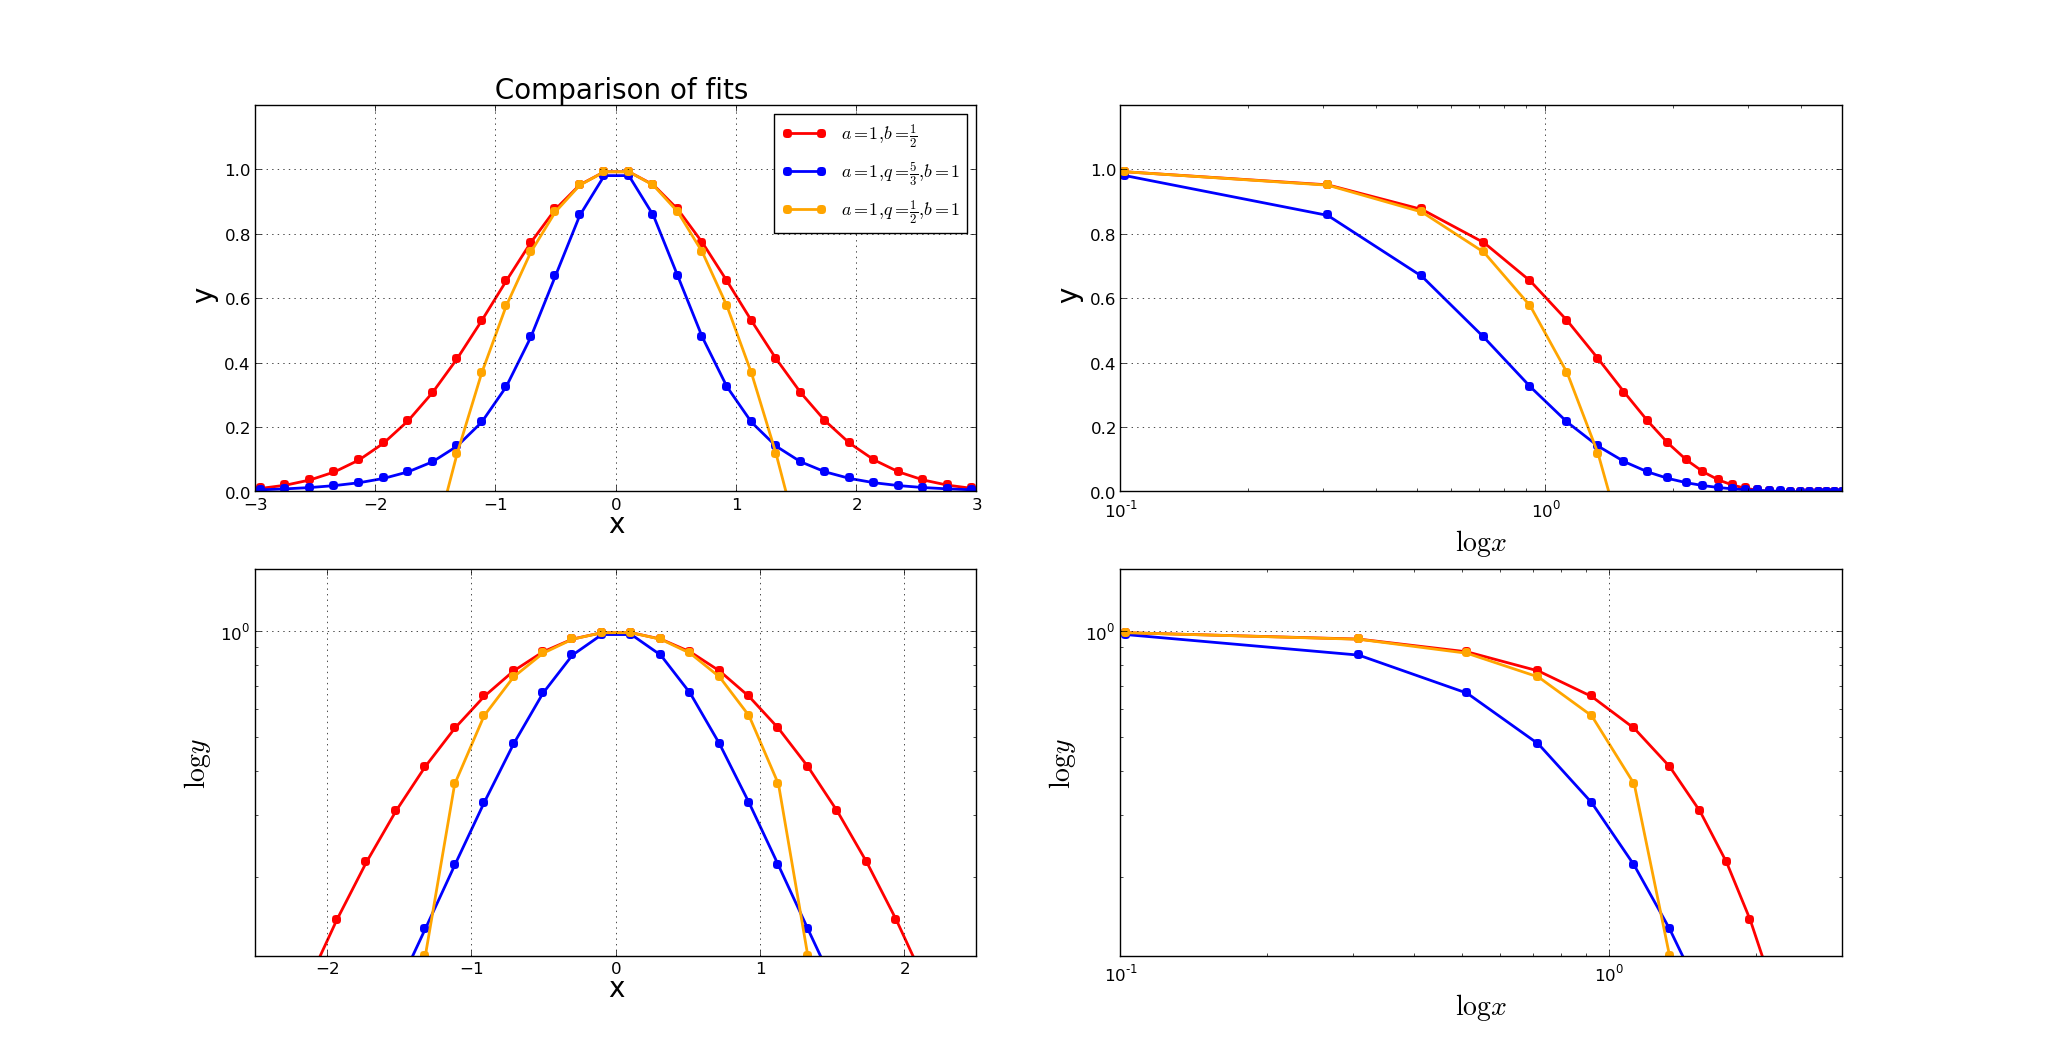
\includegraphics[width=1.0\linewidth]{img/fitcomparison.png}
\caption{$ a\cdot e^{-b\cdot x^2} $ and f(q) for $ q = \frac{5}{3}$ and $ q = \frac{1}{2}$.}
\label{fig:test}
\end{figure}

f(q) and $ae^{-bx^2}$ are both good fits to $v_{tan}$ around $\gamma = -2.0$, which is seen in figure 2:

% Tangential velocities only:
\begin{figure}
\centering
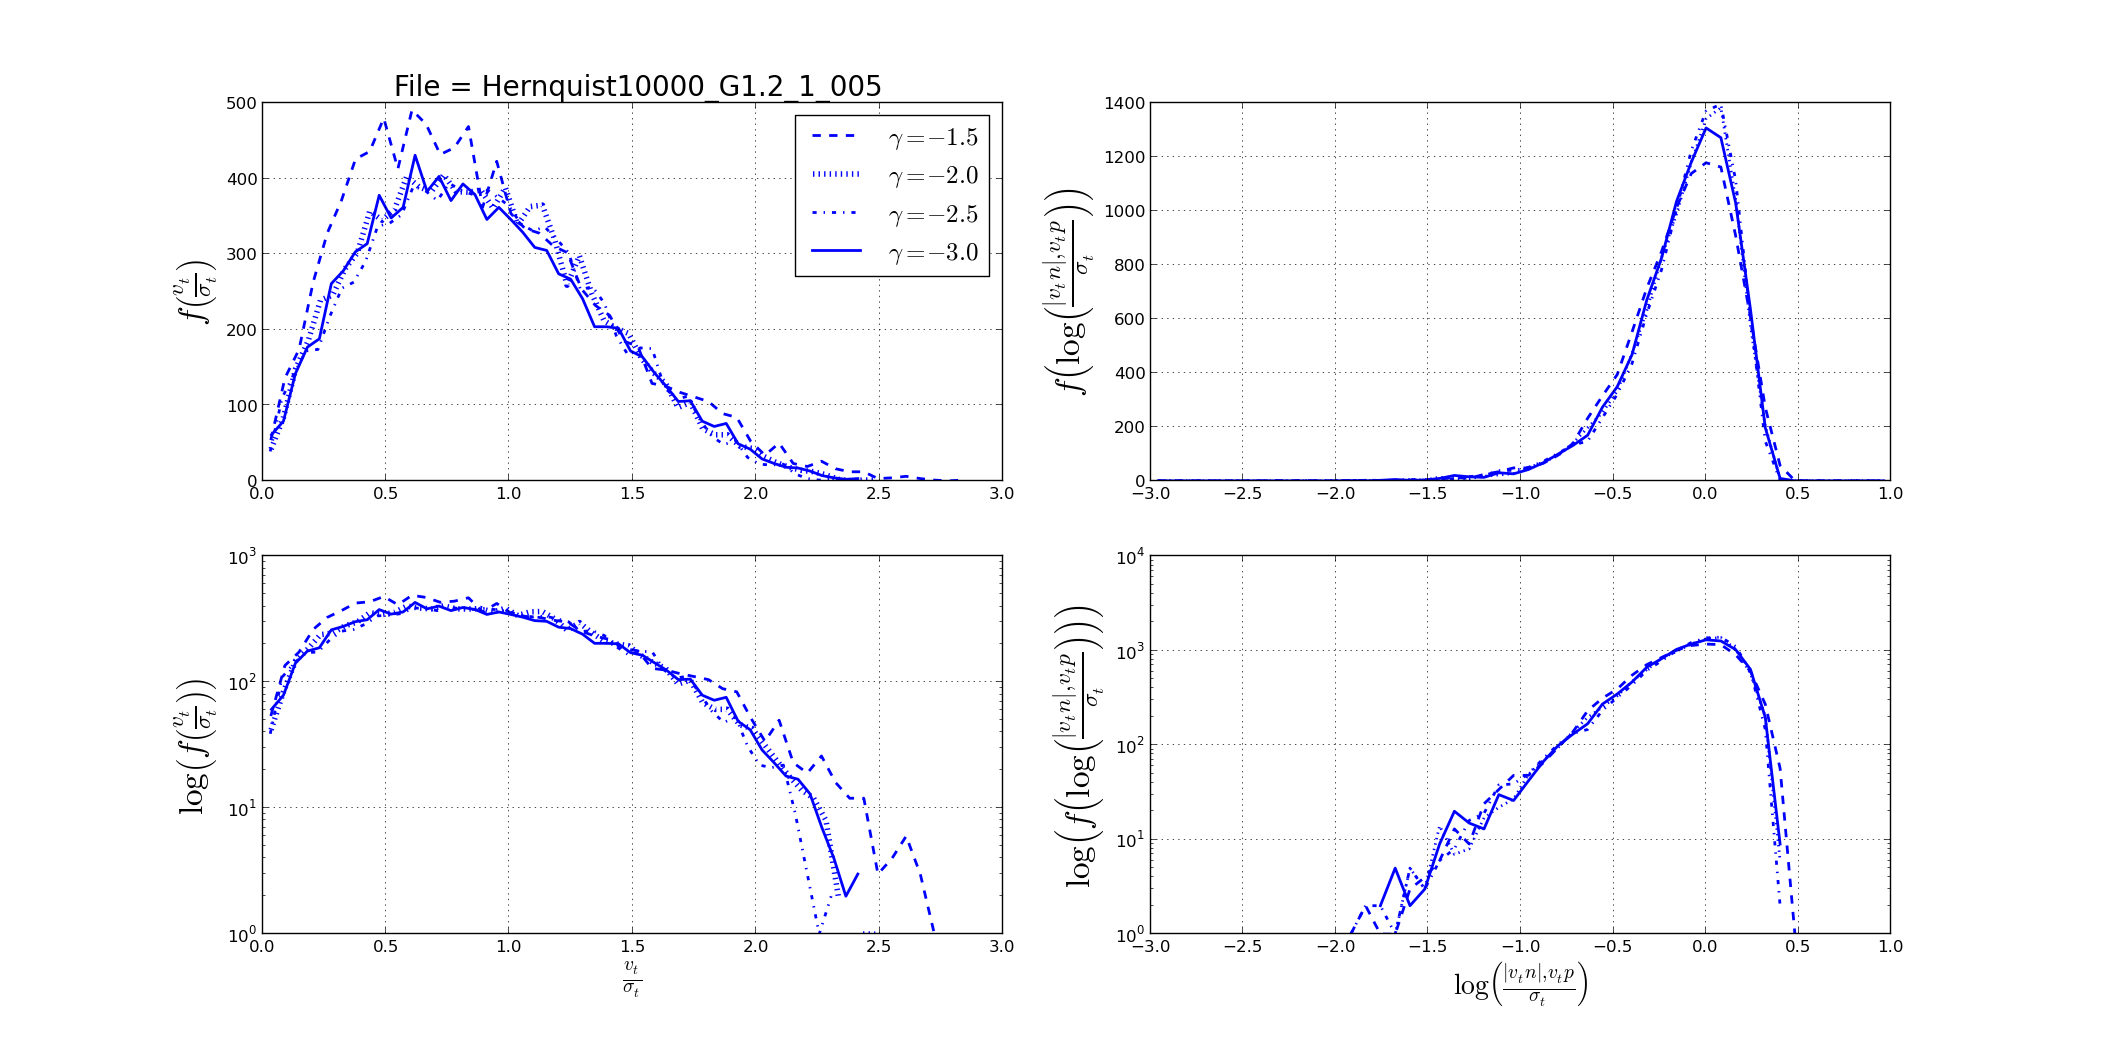
\includegraphics[width=1.0\linewidth]{img/2.png}
\caption{$v_{tan}$ divided by $\sigma_{tan}$, for 4 different radial bins. Shown in lin-lin, lin-log, log-lin and log-log}
\label{fig:test}
\end{figure}

\begin{figure}
\centering
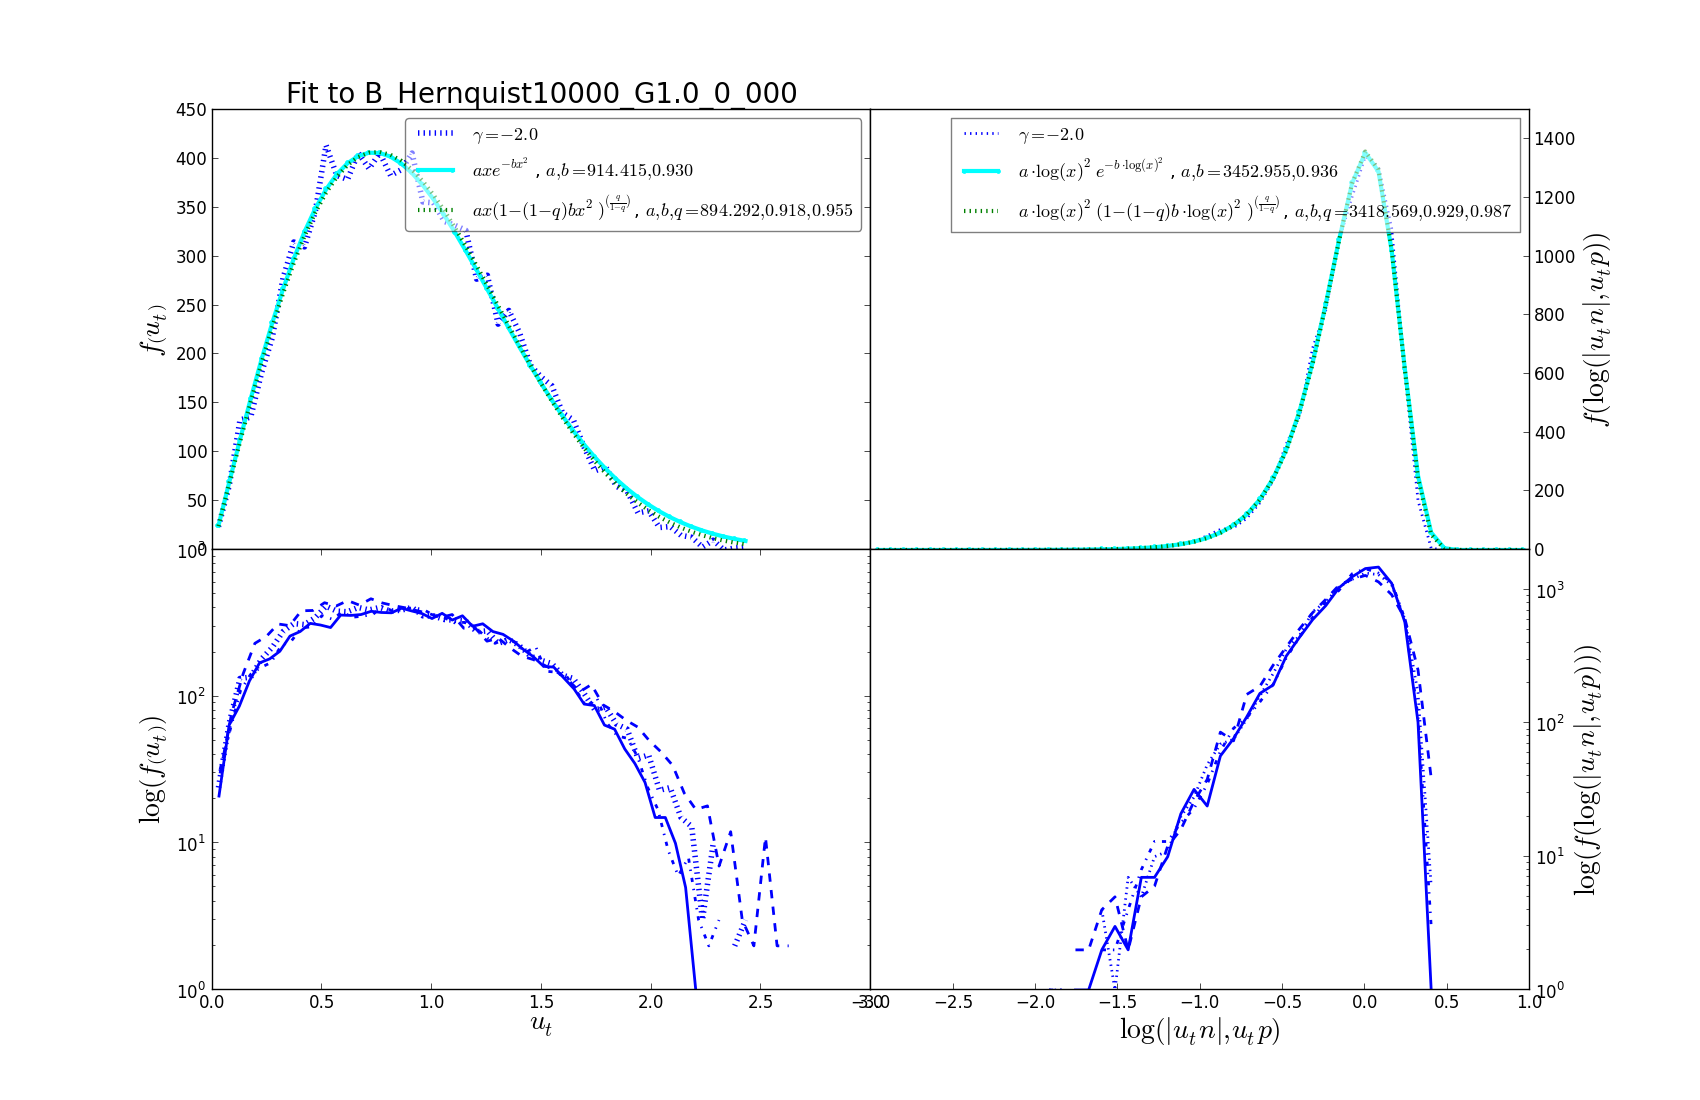
\includegraphics[width=1.0\linewidth]{img/vt_fit_show_abq.png}
\caption{$v_{tan}$ together with Gaussian and Tsallis fit.}
\label{fig:test}
\end{figure}

\begin{figure}
\centering
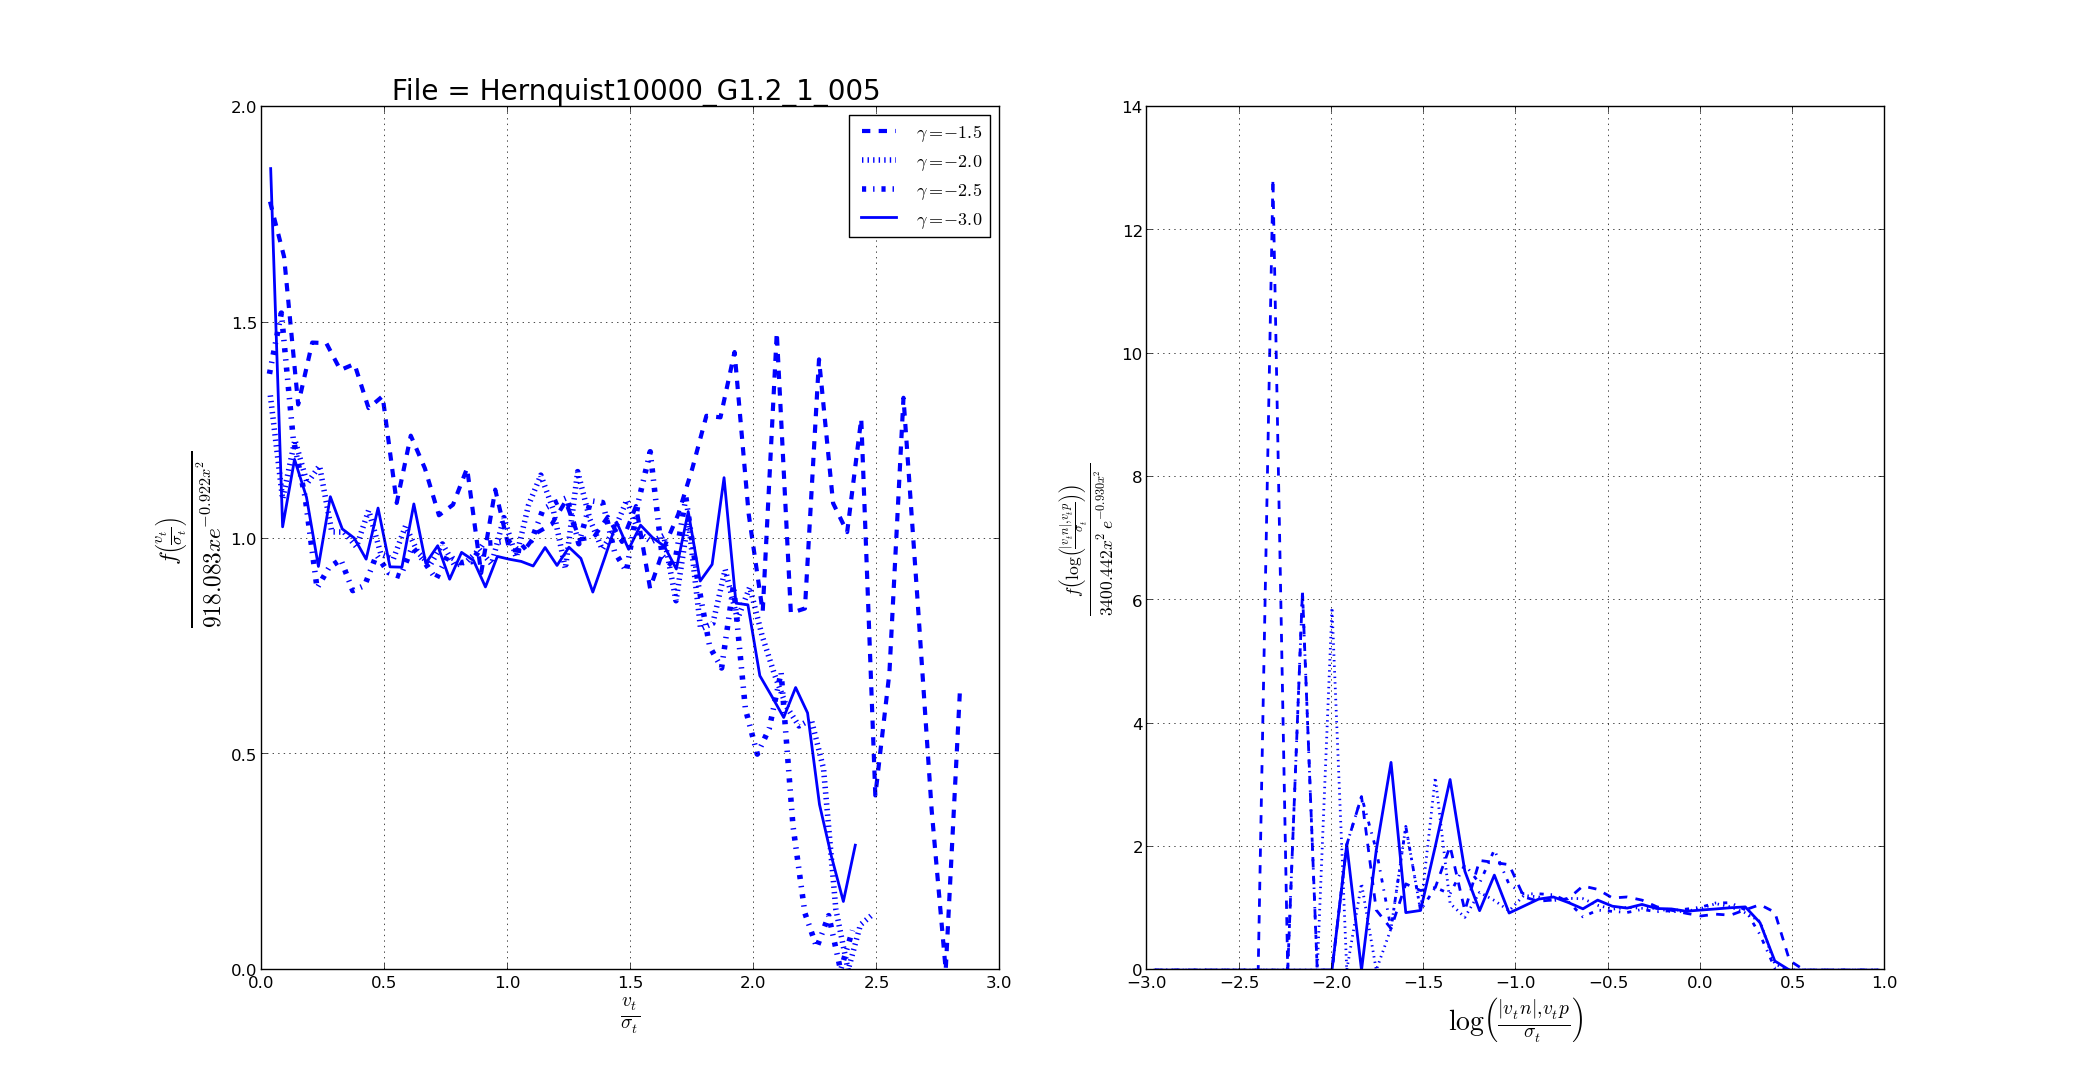
\includegraphics[width=1.0\linewidth]{img/func_guess_vt.png}
\caption{$v_{tan}$ divided by Gaussian function.}
\label{fig:test}
\end{figure}

\begin{figure}
\centering
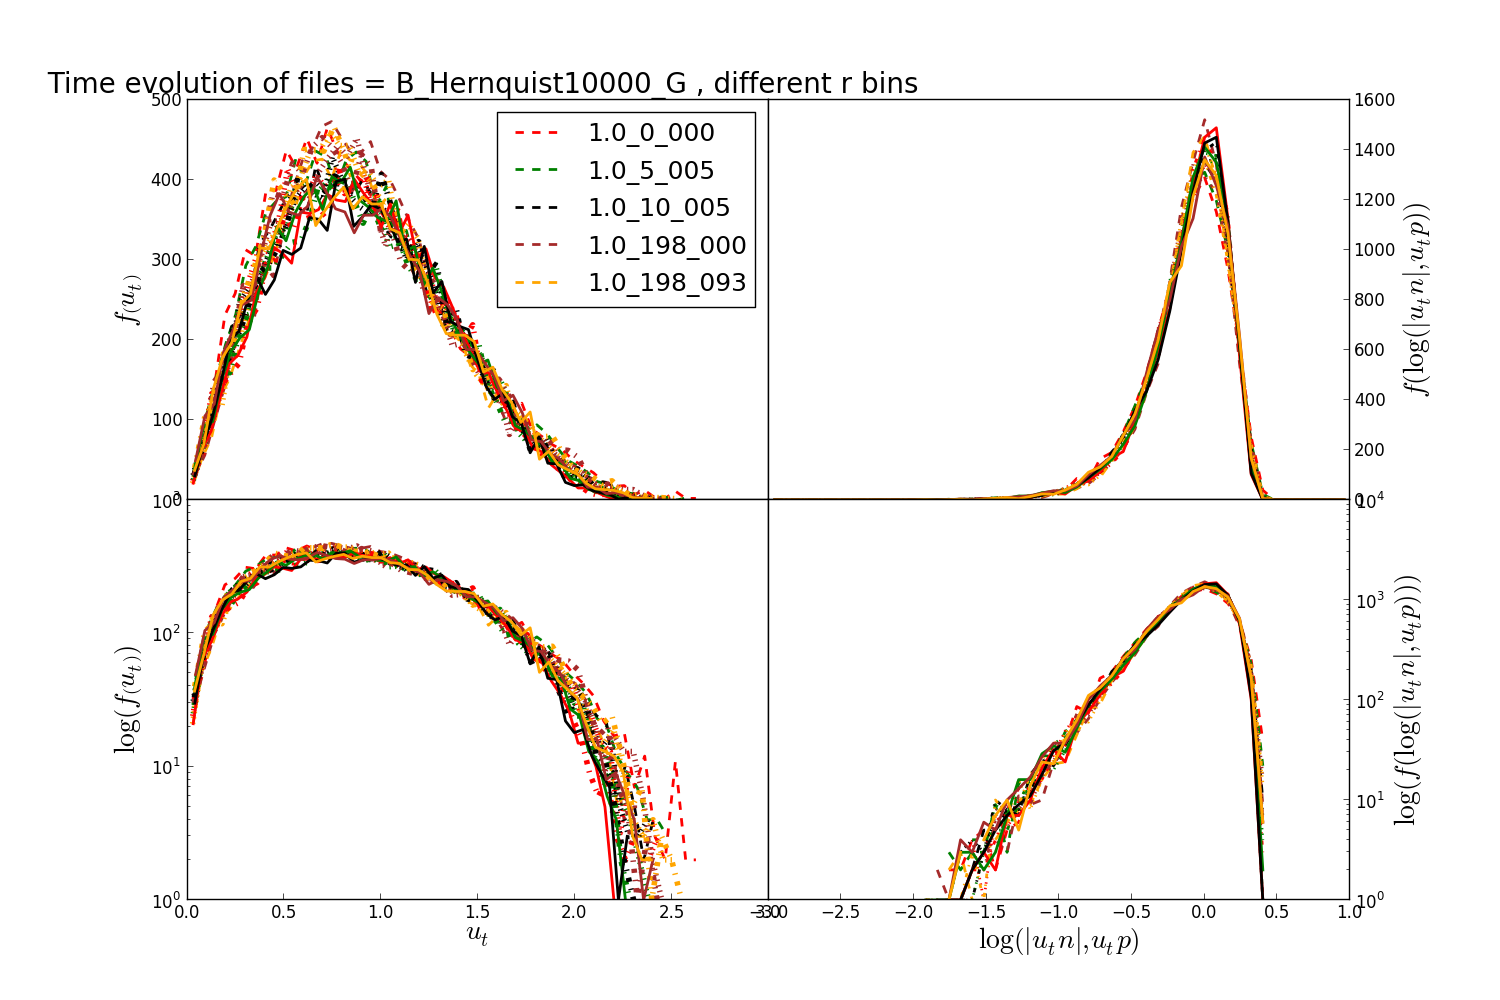
\includegraphics[width=1.0\linewidth]{img/Time_evolution_B_vt_different_rbins.png}
\caption{Histograms of the ratio $ u_t = \frac{v_{tan}}{\sigma_{tan}} $ for 5 different snapshots (this makes it easier to compare different radial bins than it would be for $ v_{tan} $ alone). Data for 4 different radial bins are shown, each containing $10^4$ particles and centered at the radii where $\gamma = -1.5, -2.0, -2.5 $ and $-3.0 $ respectively.}
\label{fig:test}
\end{figure}

% Radial, theta and phi velocities:

\begin{figure}
\centering
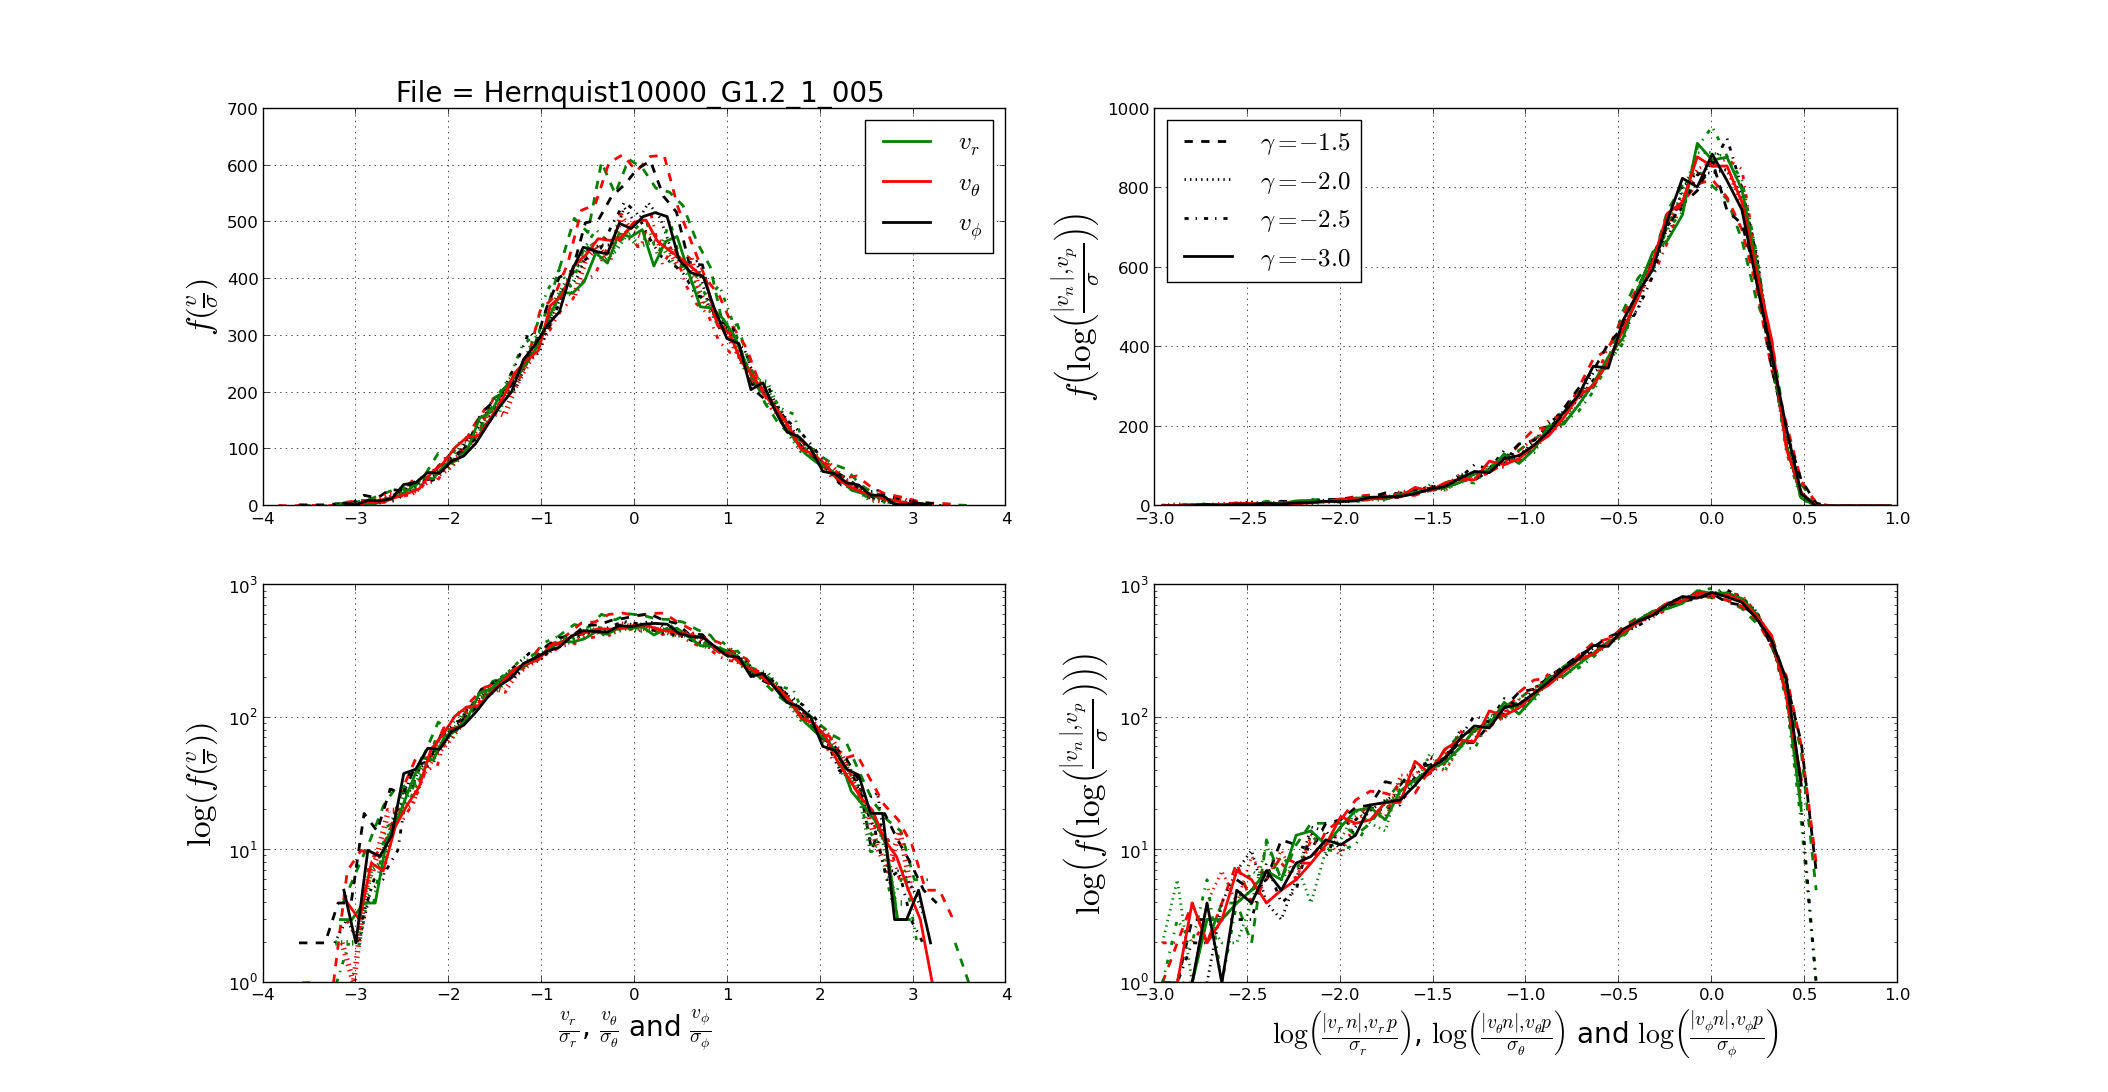
\includegraphics[width=1.0\linewidth]{img/1.png}
\caption{$v_{r}$, $v_{\theta}$ and $v_{\phi}$ divided by $\sigma_{r}$, $\sigma_{\theta}$ and $\sigma_{\phi}$ respectively, for 4 different radial bins. Shown in lin-lin, lin-log, log-lin and log-log}
\label{fig:test}
\end{figure}

\begin{figure}
\centering
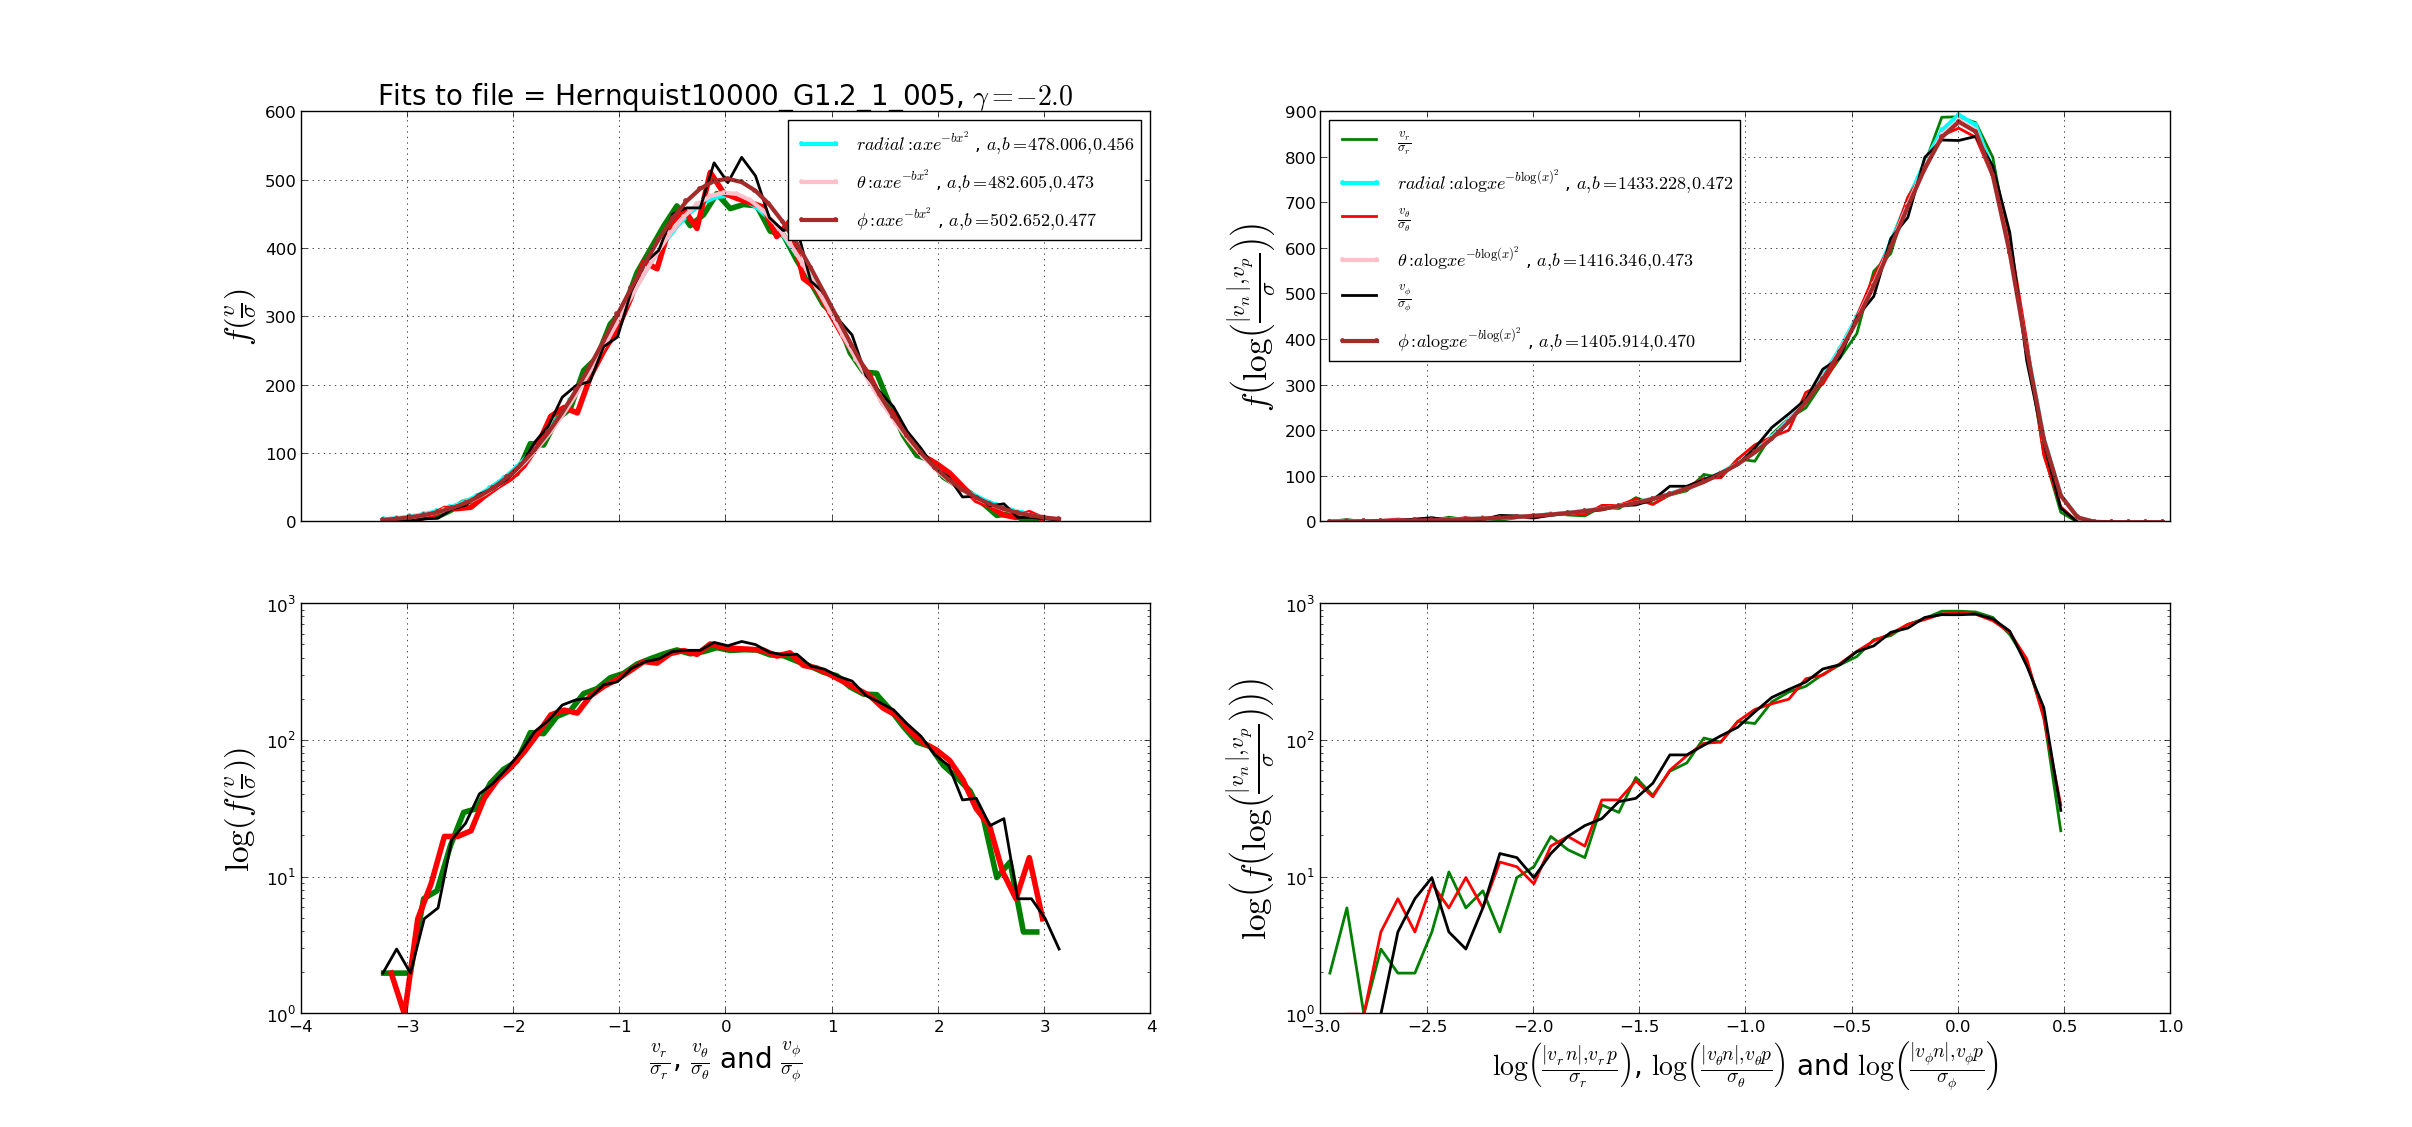
\includegraphics[width=1.0\linewidth]{img/vr_vtheta_vphi_fit.png}
\caption{$v_{r}$, $v_{\theta}$ and $v_{\phi}$ together with Gaussian and Tsallis fit.}
\label{fig:test}
\end{figure}

\begin{figure}
\centering
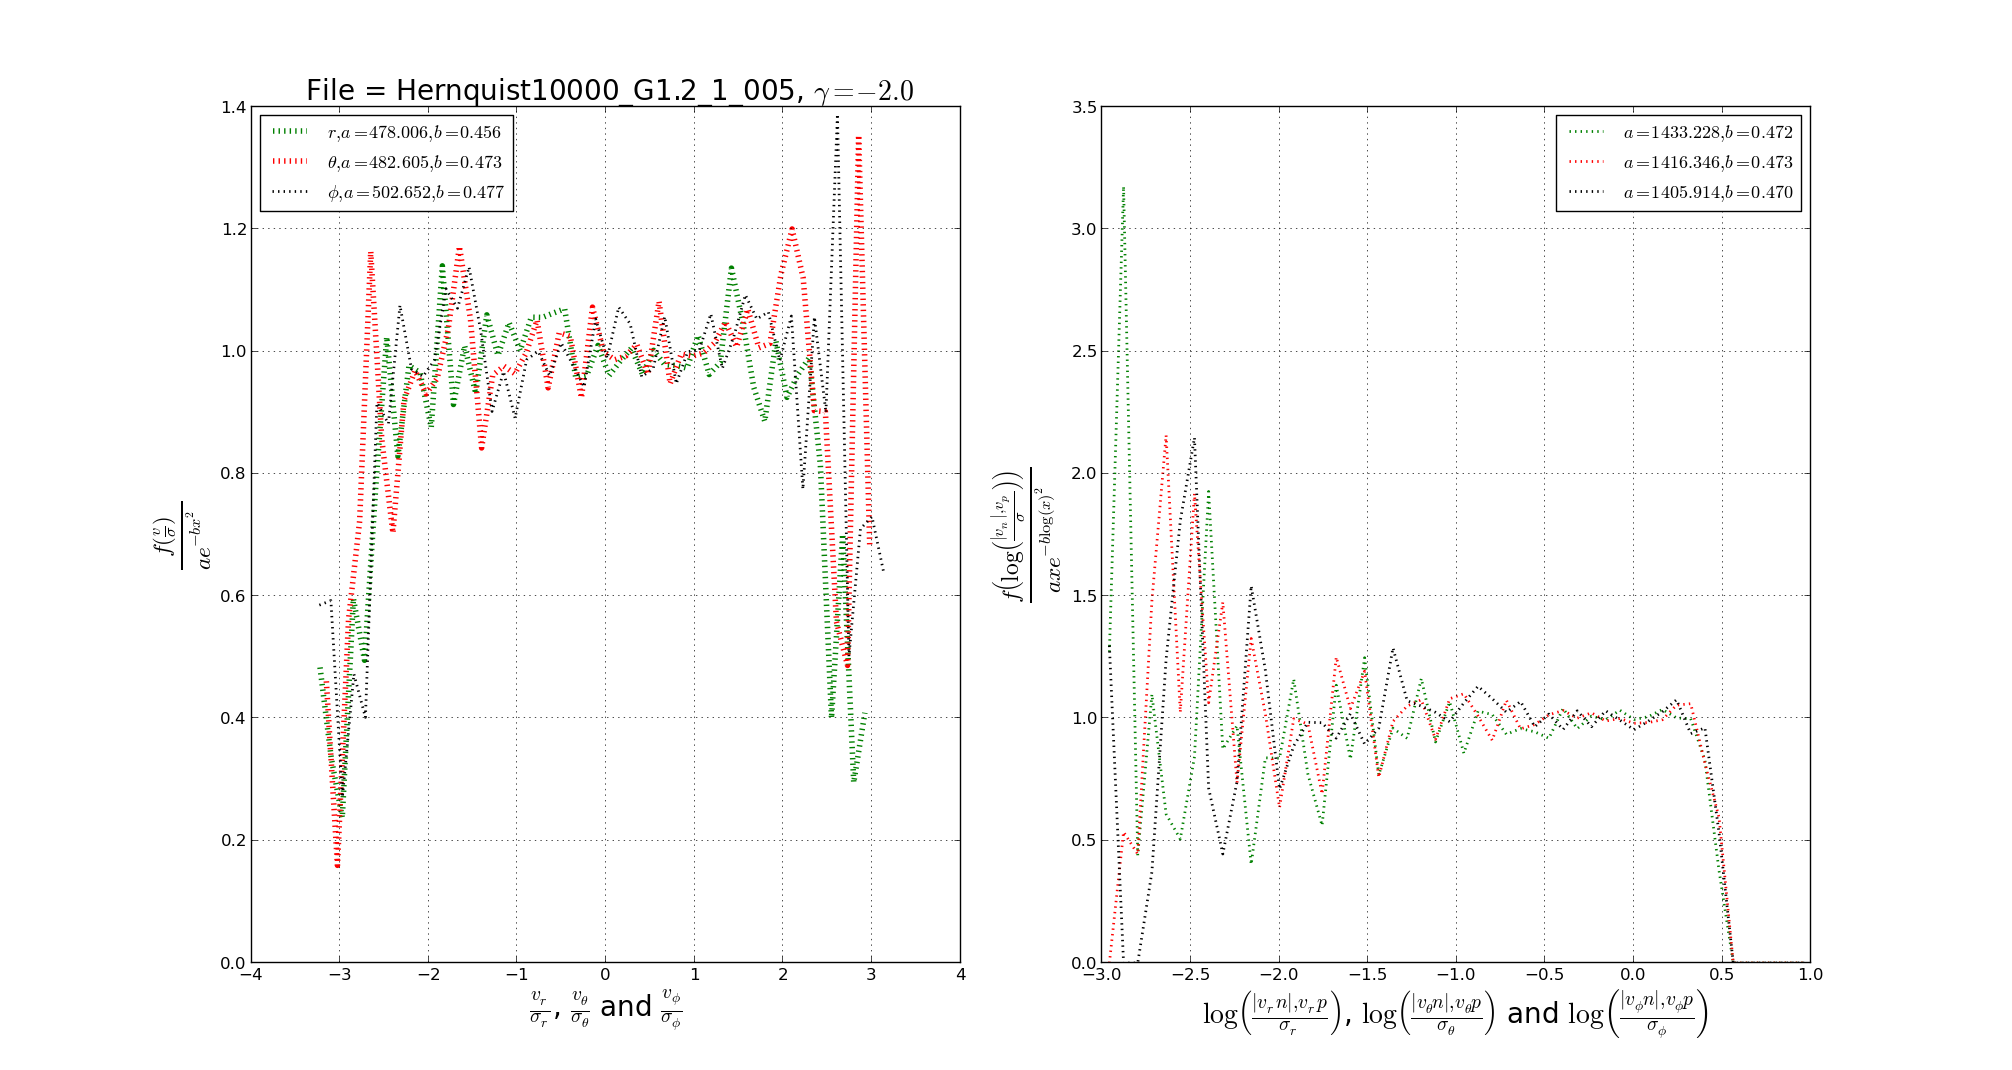
\includegraphics[width=1.0\linewidth]{img/func_guess_vr_vtheta_vphi.png}
\caption{$v_{r}$, $v_{\theta}$ and $v_{\phi}$ divided by Gaussian function.}
\label{fig:test}
\end{figure}

\newpage
\subsection{Line-of-sight overdensities}
Starting with an end-product from a G-perturbation simulation, which is no longer perfectly spherical and therefore more closely resembles a cosmological DM halo, a plot of radial velocity, $v_r$ vs. radius, r (for a 3D simulation file) is compared to the corresponding plot of velocity along the x-direction, $v_x$ (taken to be the line-of-sight, LOS) vs the projected radius, R (given by $R = \sqrt{y^2+z^2}$).
It is possible to simulate 3D structures, but in reality it is only possible to observe the LOS-velocity, $v_{LOS}$ here defined to be $v_x$. R is the projected radius onto LOS and r is here the 3D radius vector from the simulation.
An interesting question to investigate is: How does overdensities in 3D look in this corresponding 2D representation ($v_x$ vs $R$)?

%\begin{figure}
%\centering
%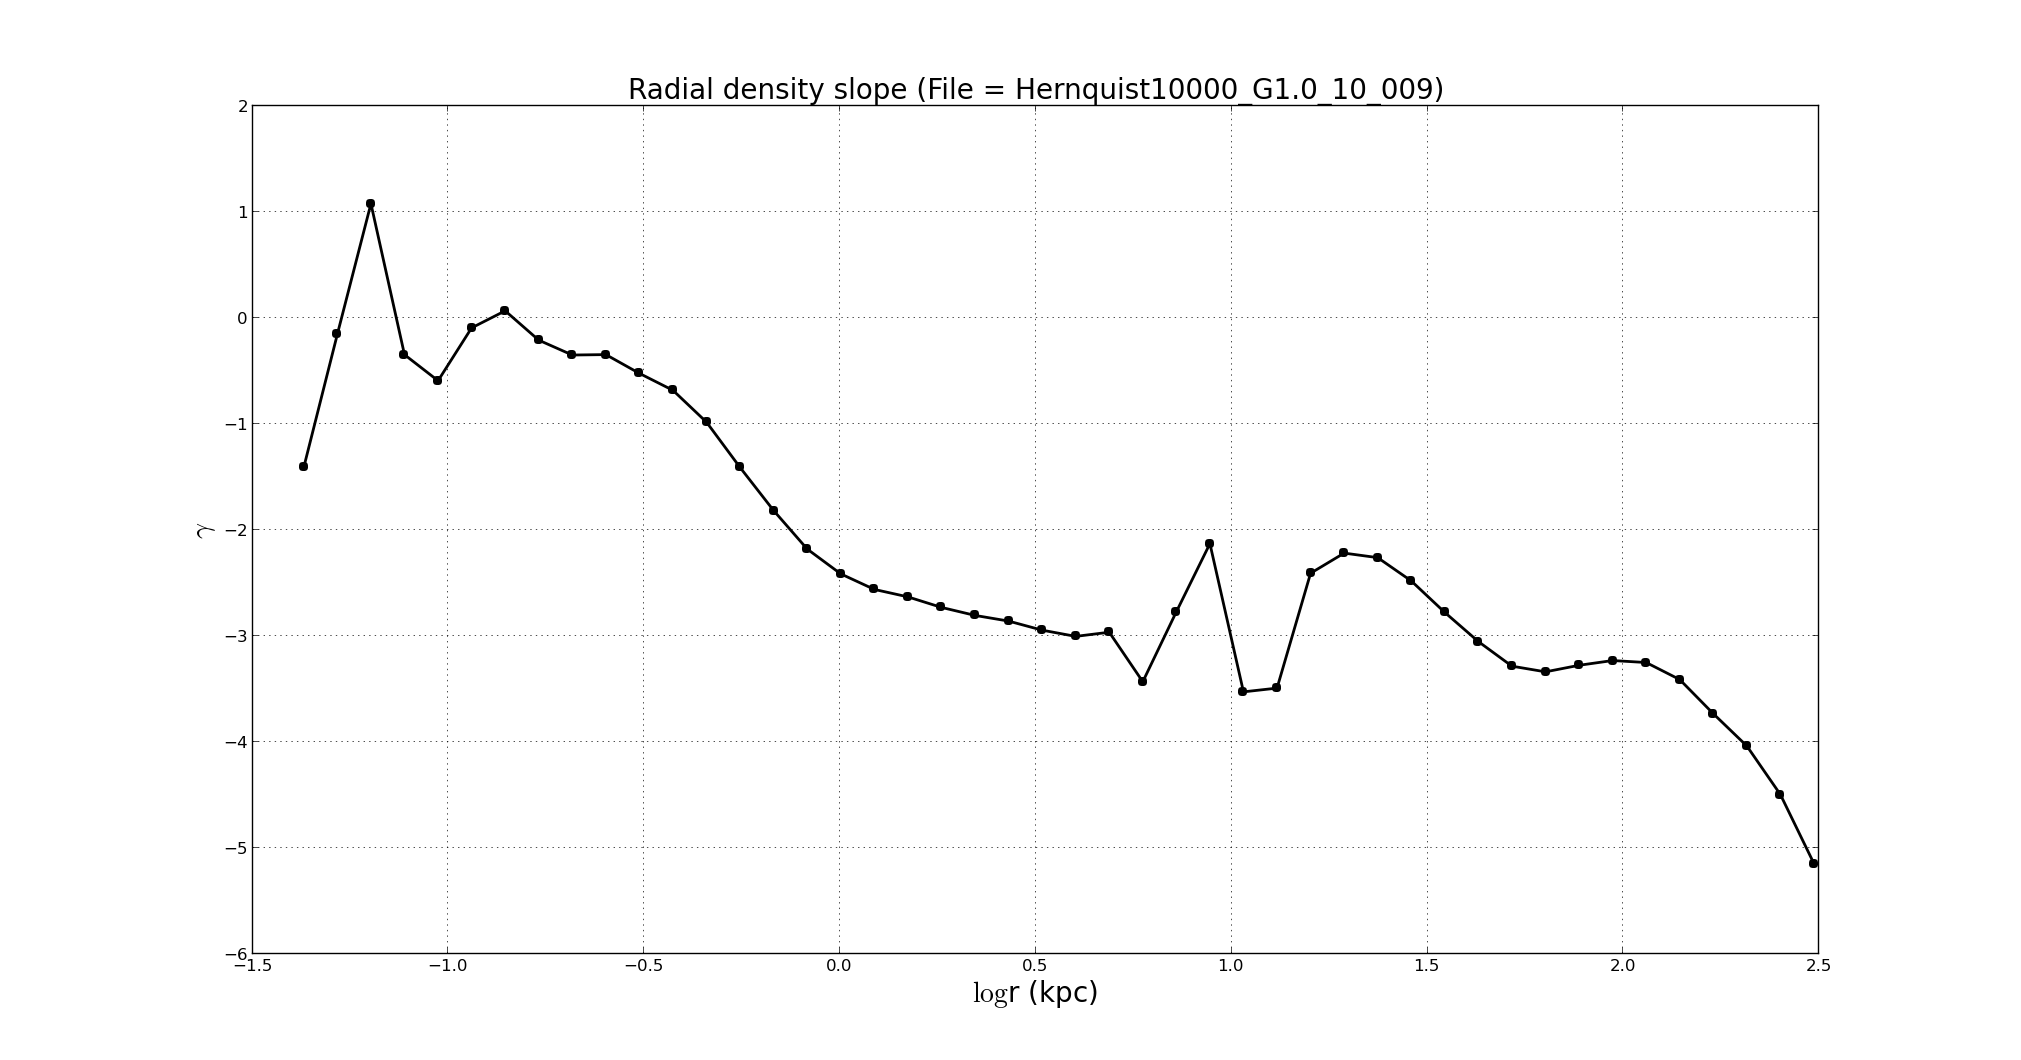
\includegraphics[width=1.0\linewidth]{img/endproduct_gamma.png}
%\caption{}
%\label{fig:test}
%\end{figure}

%\begin{figure}
%\centering
%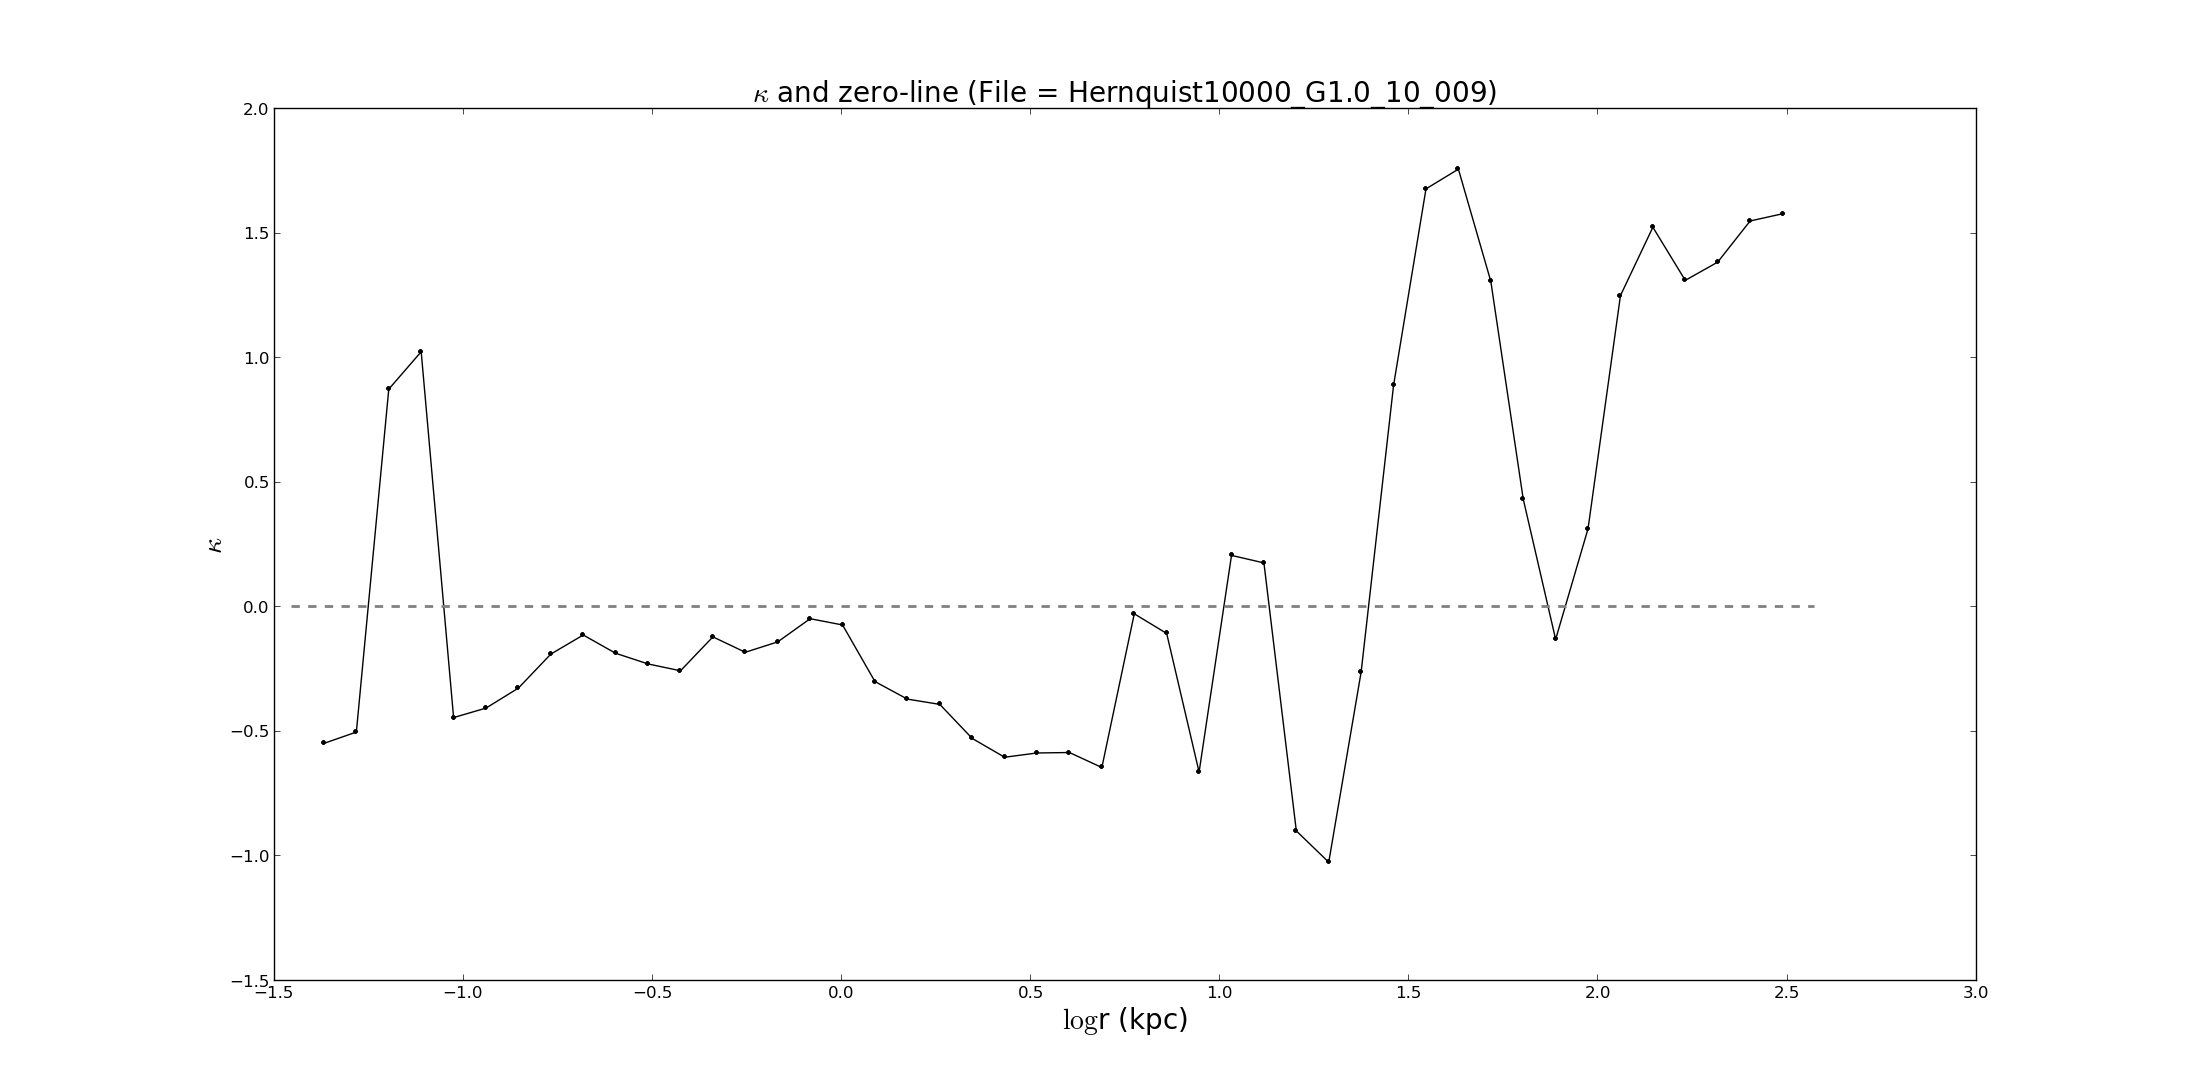
\includegraphics[width=1.0\linewidth]{img/endproduct_kappa.png}
%\caption{}
%\label{fig:test}
%\end{figure}

%\begin{figure}
%\centering
%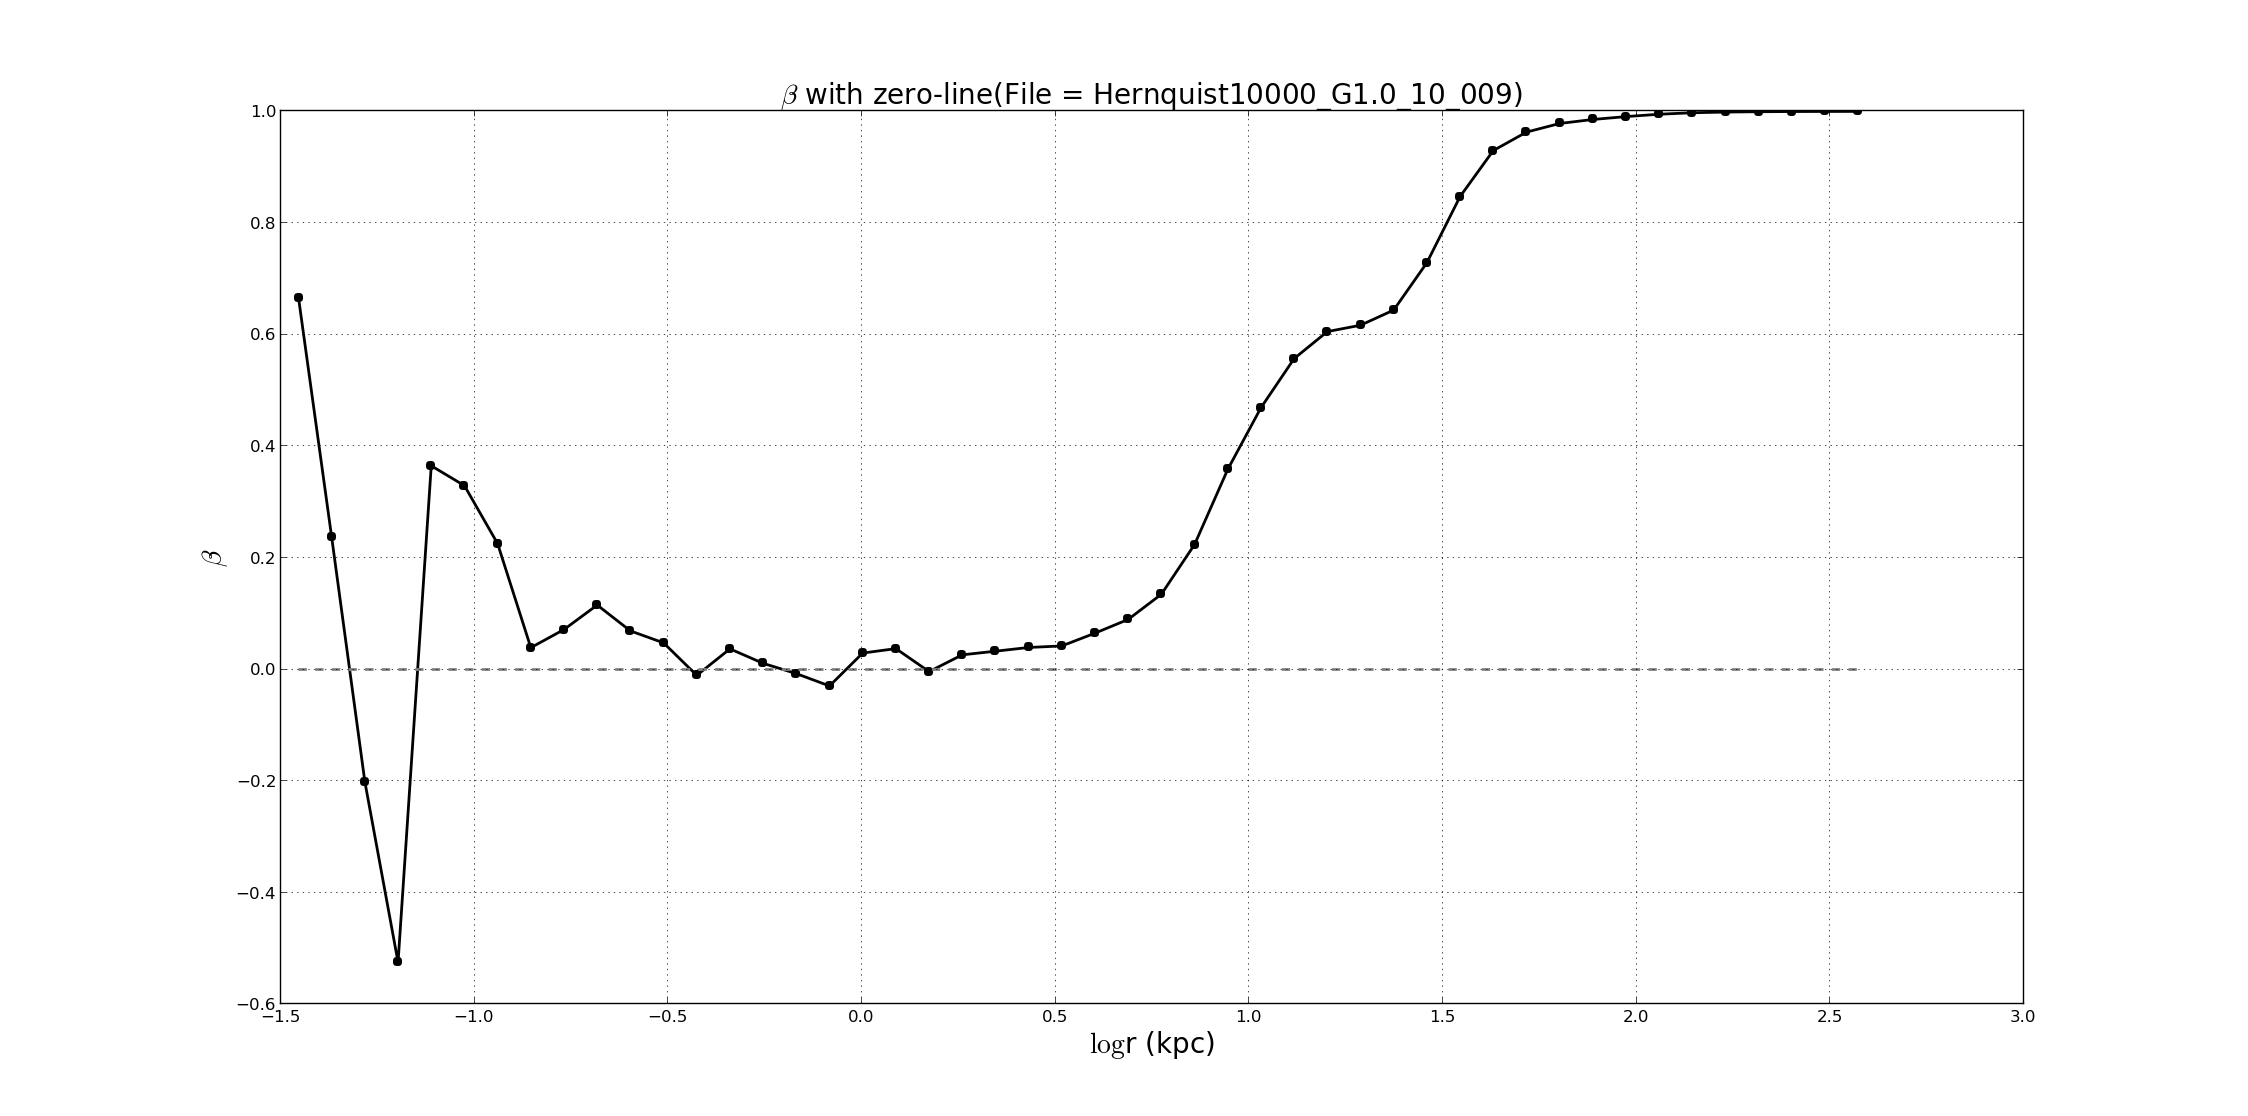
\includegraphics[width=1.0\linewidth]{img/endproduct_beta.png}
%\caption{}
%\label{fig:test}
%\end{figure}

%\begin{figure}
%\centering
%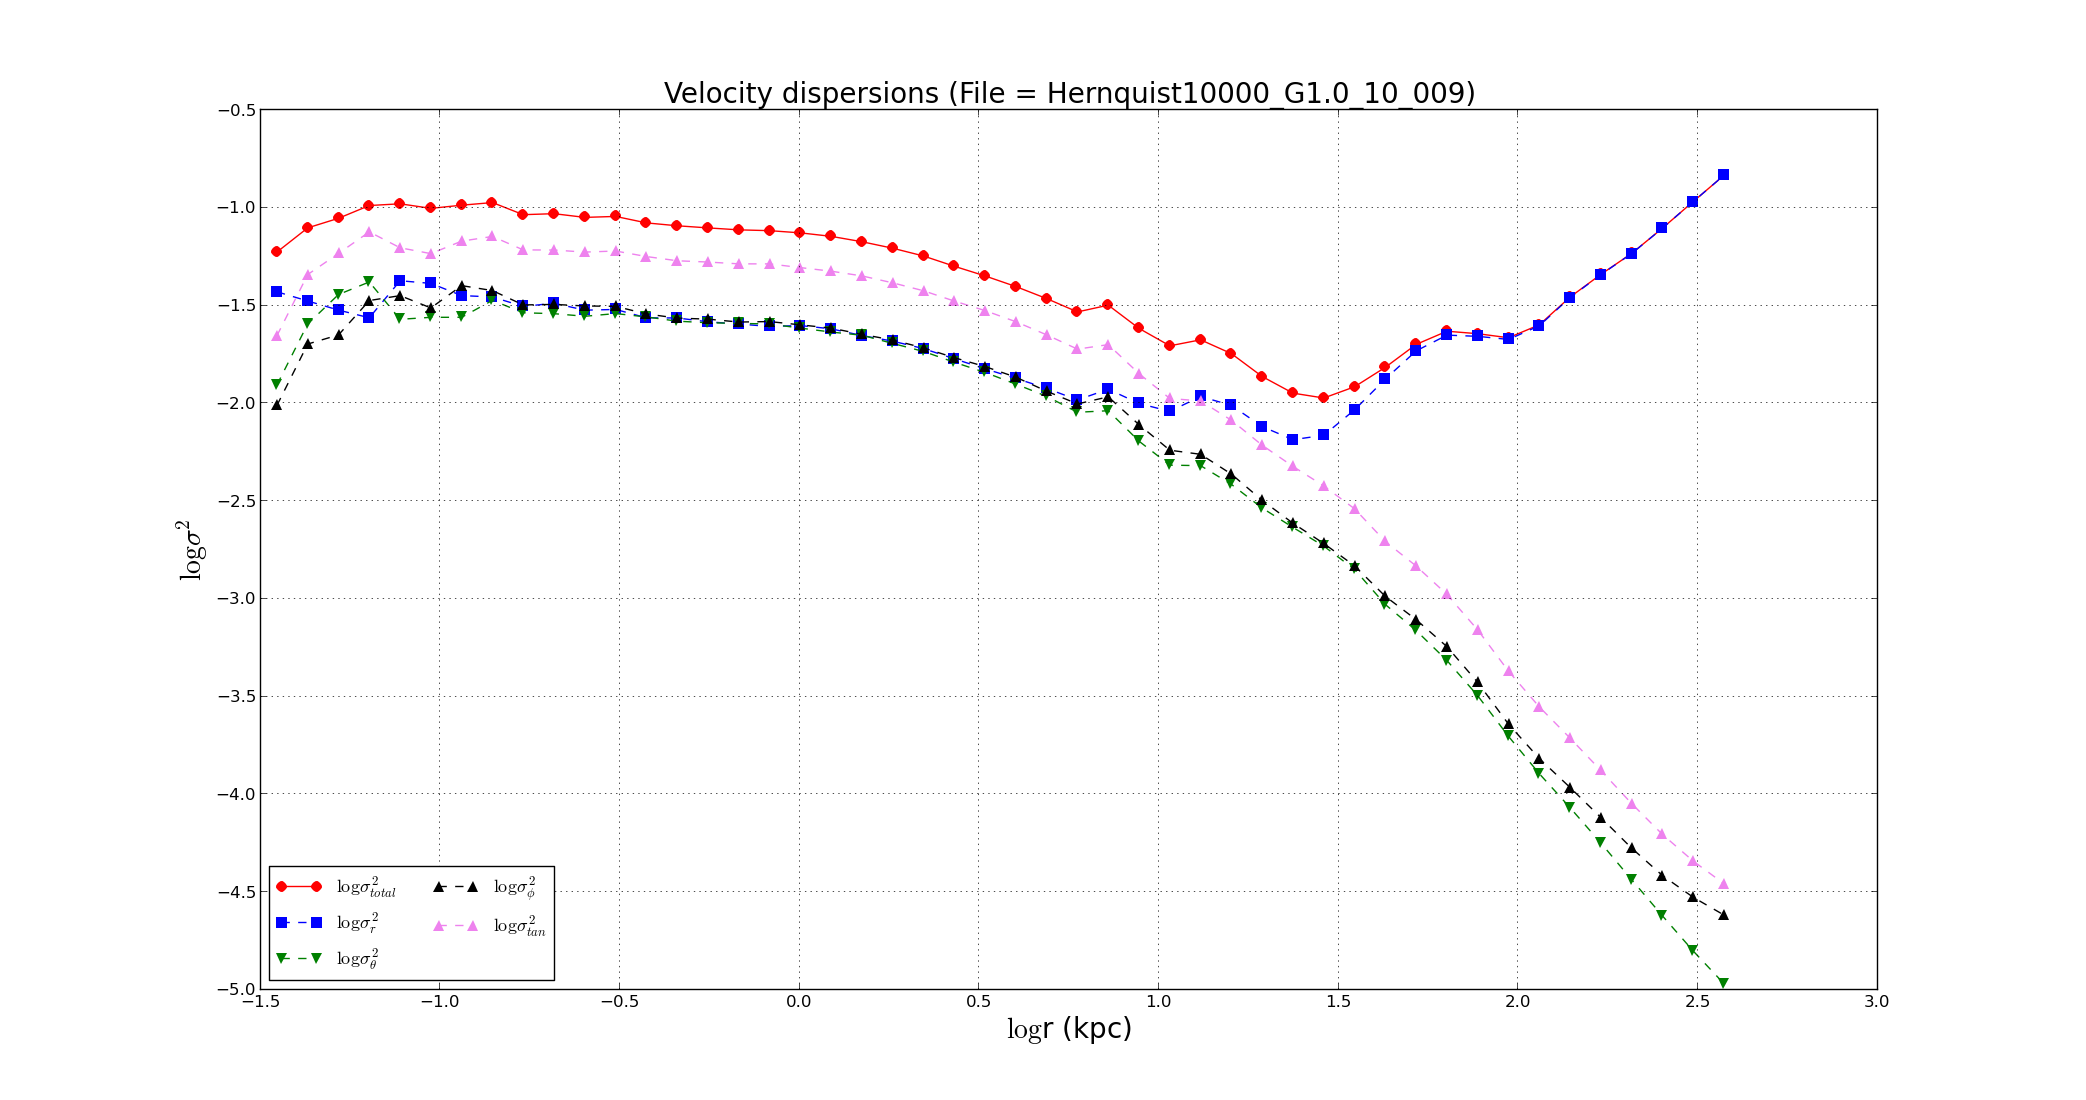
\includegraphics[width=1.0\linewidth]{img/endproduct_sigmas.png}
%\caption{}
%\label{fig:test}
%\end{figure}

%\begin{figure}
%\centering
%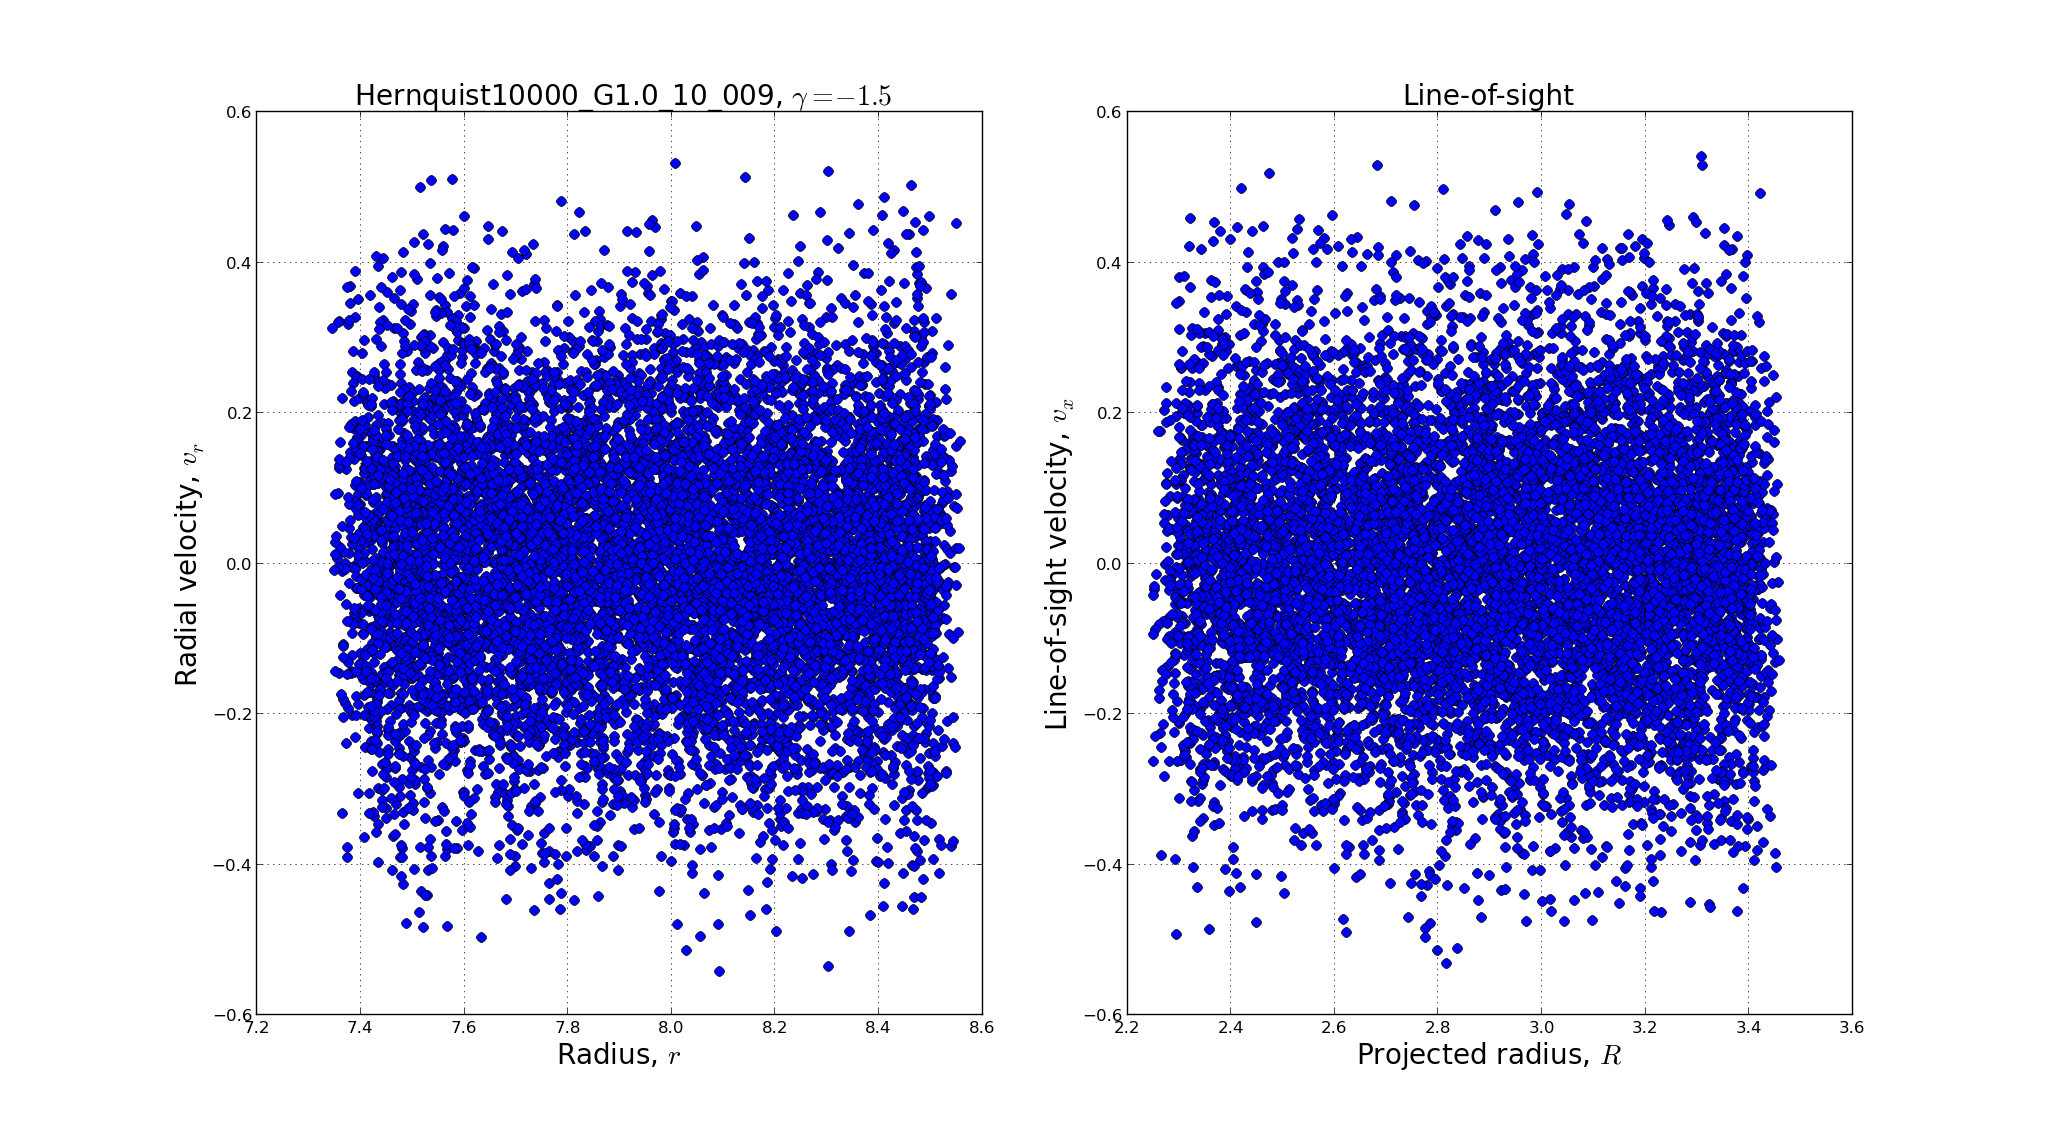
\includegraphics[width=1.0\linewidth]{img/LOS_gammaminus1_5.png}
%\caption{For the file Hernquist10000\_G1.0\_10\_009 we here see a comparison of the radial velocity as function of radius (left panel)
%to the LOS-velocity vs the projected radius. It is shown for a radial bin containing $10^4$ particles, centered around the radius where $\gamma = -1.5$}
%\label{fig:test}
%\end{figure}

%\begin{figure}
%\centering
%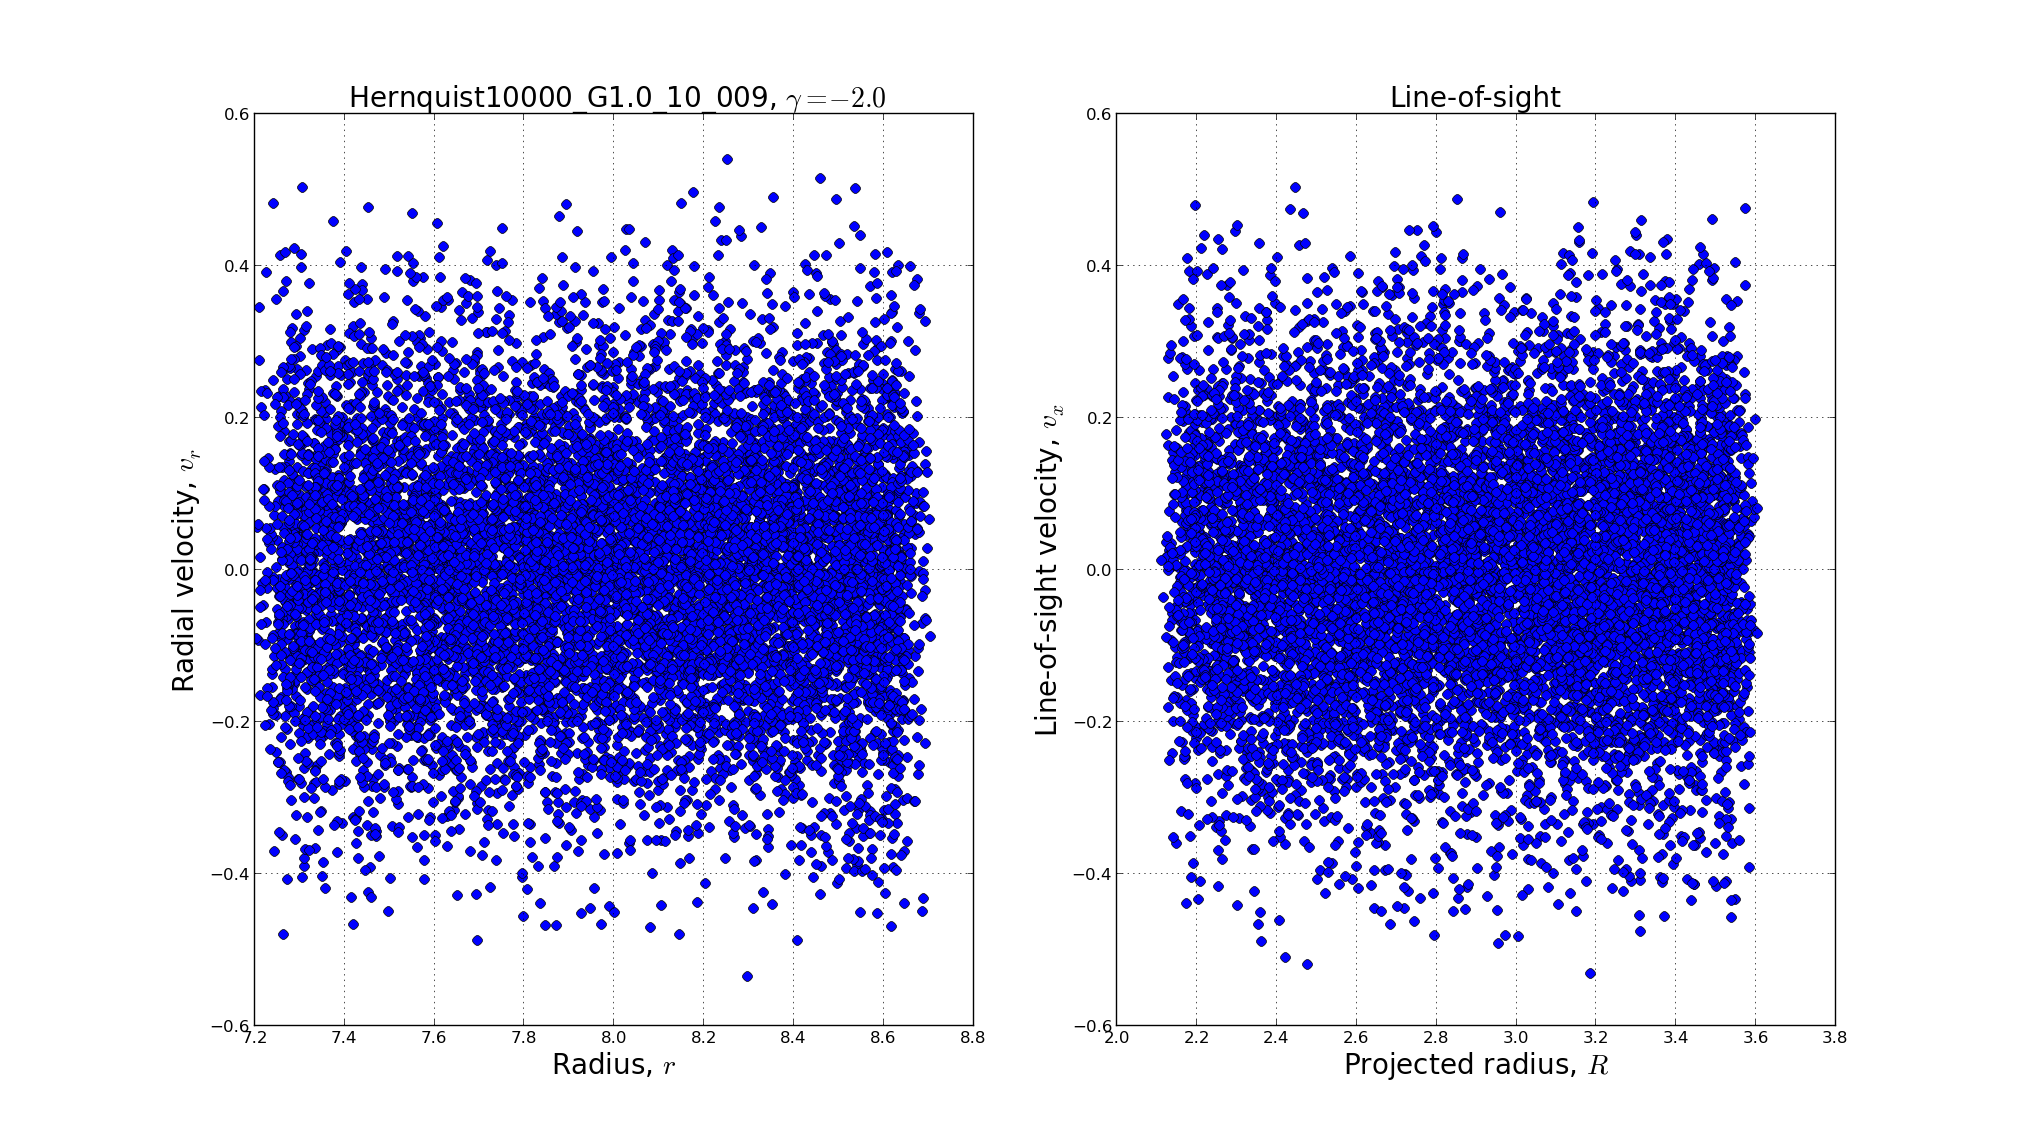
\includegraphics[width=1.0\linewidth]{img/LOS_gammaminus2_0.png}
%\caption{For the file Hernquist10000$\_$G1.0$\_$10$\_$009 we here see a comparison of the radial velocity as function of radius (left panel)
%to the LOS-velocity vs the projected radius. It is shown for a radial bin containing $10^4$ particles, centered around the radius where $\gamma = -2.0$}
%\label{fig:test}
%\end{figure}

\begin{figure}
\centering
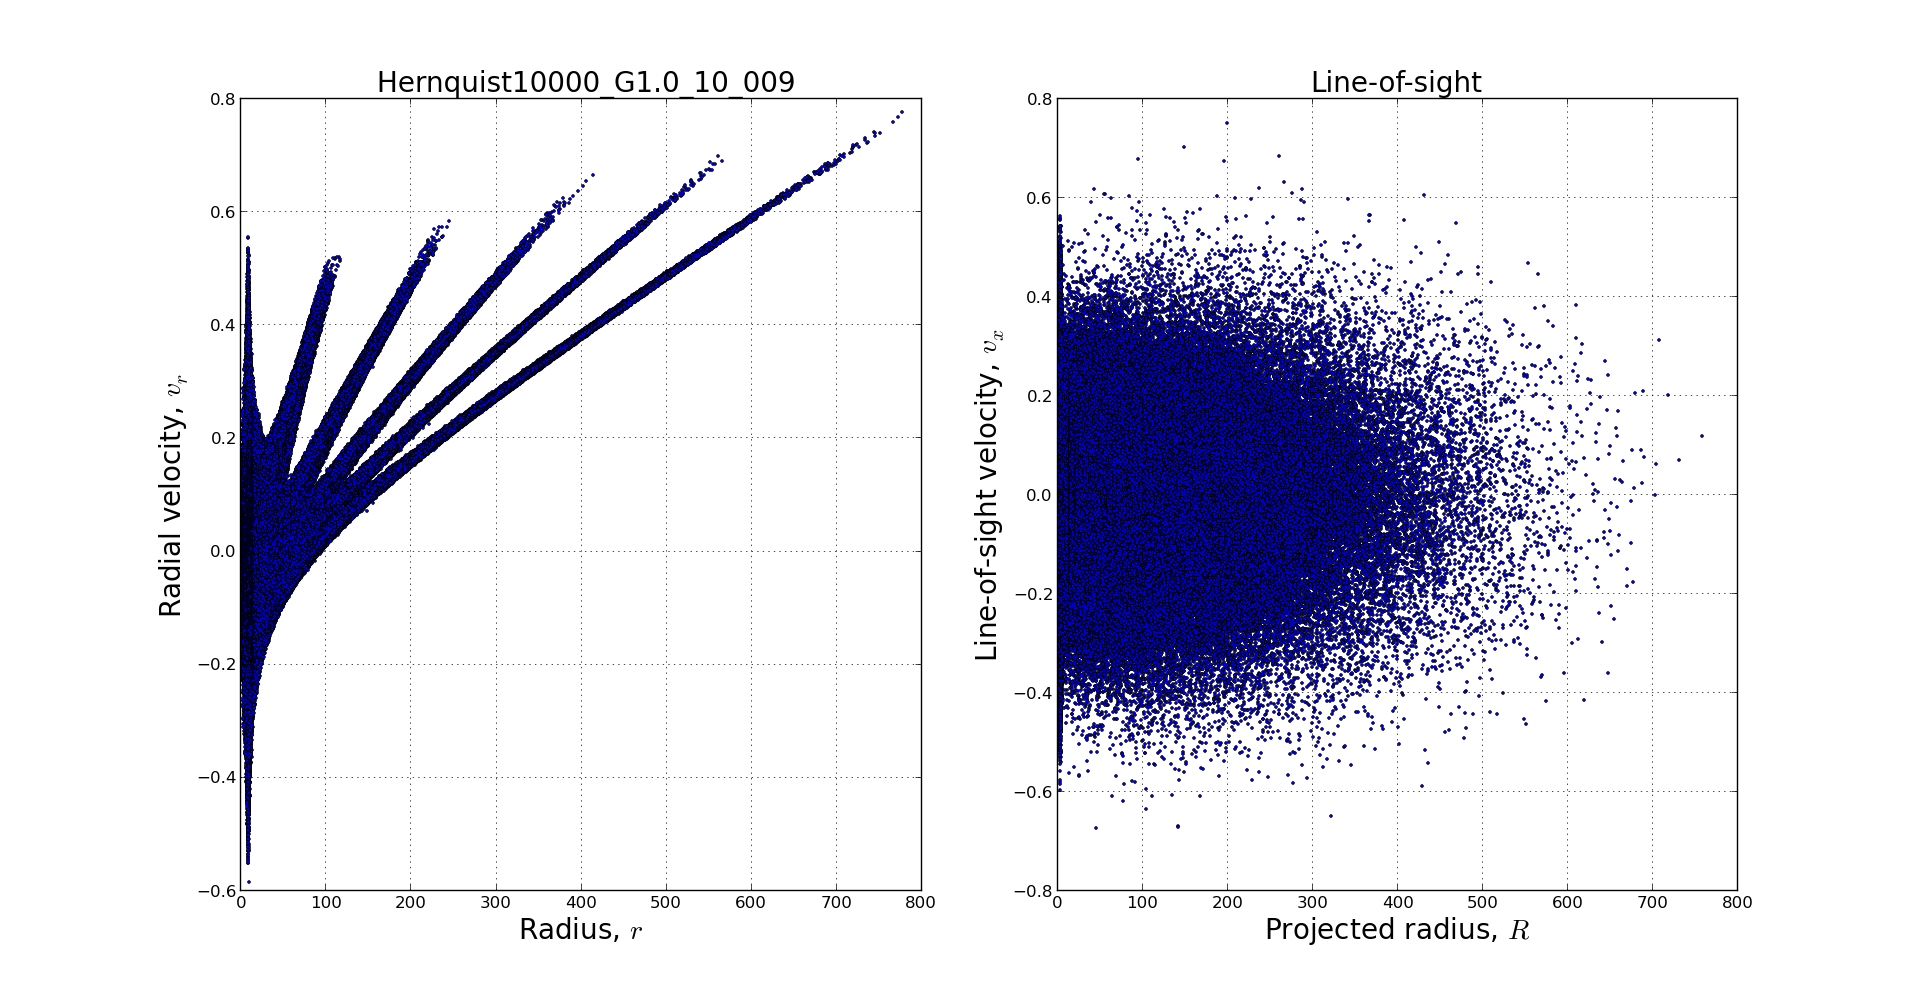
\includegraphics[width=1.0\linewidth]{img/LOS.png}
\caption{For the file Hernquist10000$\_$G1.0$\_$10$\_$009 containing $10^6$ particles we here see a comparison of the radial velocity as function of radius (left panel) to the LOS-velocity vs the projected radius for the G-perturbation simulation. The left panel showing the radial velocity clearly portrays the presence of substructure which is washed out in the corresponding line-of-sight plot in the right plot. This point makes it clear that numerical simulations can provide a full picture absent when performing observations naturally restricted to the line of sight. The radial velocity plot has 5 distinct filaments, one for each of the perturbations. The filament furthest to the right corresponds to the first time particles escapes the structure.}
\label{fig:test}
\end{figure}

The biggest difference between the $r, v_r$-graph and the $R, v_x$-graph is the amount of information lost when going from 3D quantities to line-of-sight quantities.
Notice in particular the high degree of substructure in the $r, v_r$-graph;
we see 5 arms corresponding to each variation of G, which is in a way frozen into the phase-space volume. When G is increased, the radial velocity grows rapidly for larger radii, and when G is decreased, the radial velocity falls off just as rapid. 

\begin{figure}
\centering
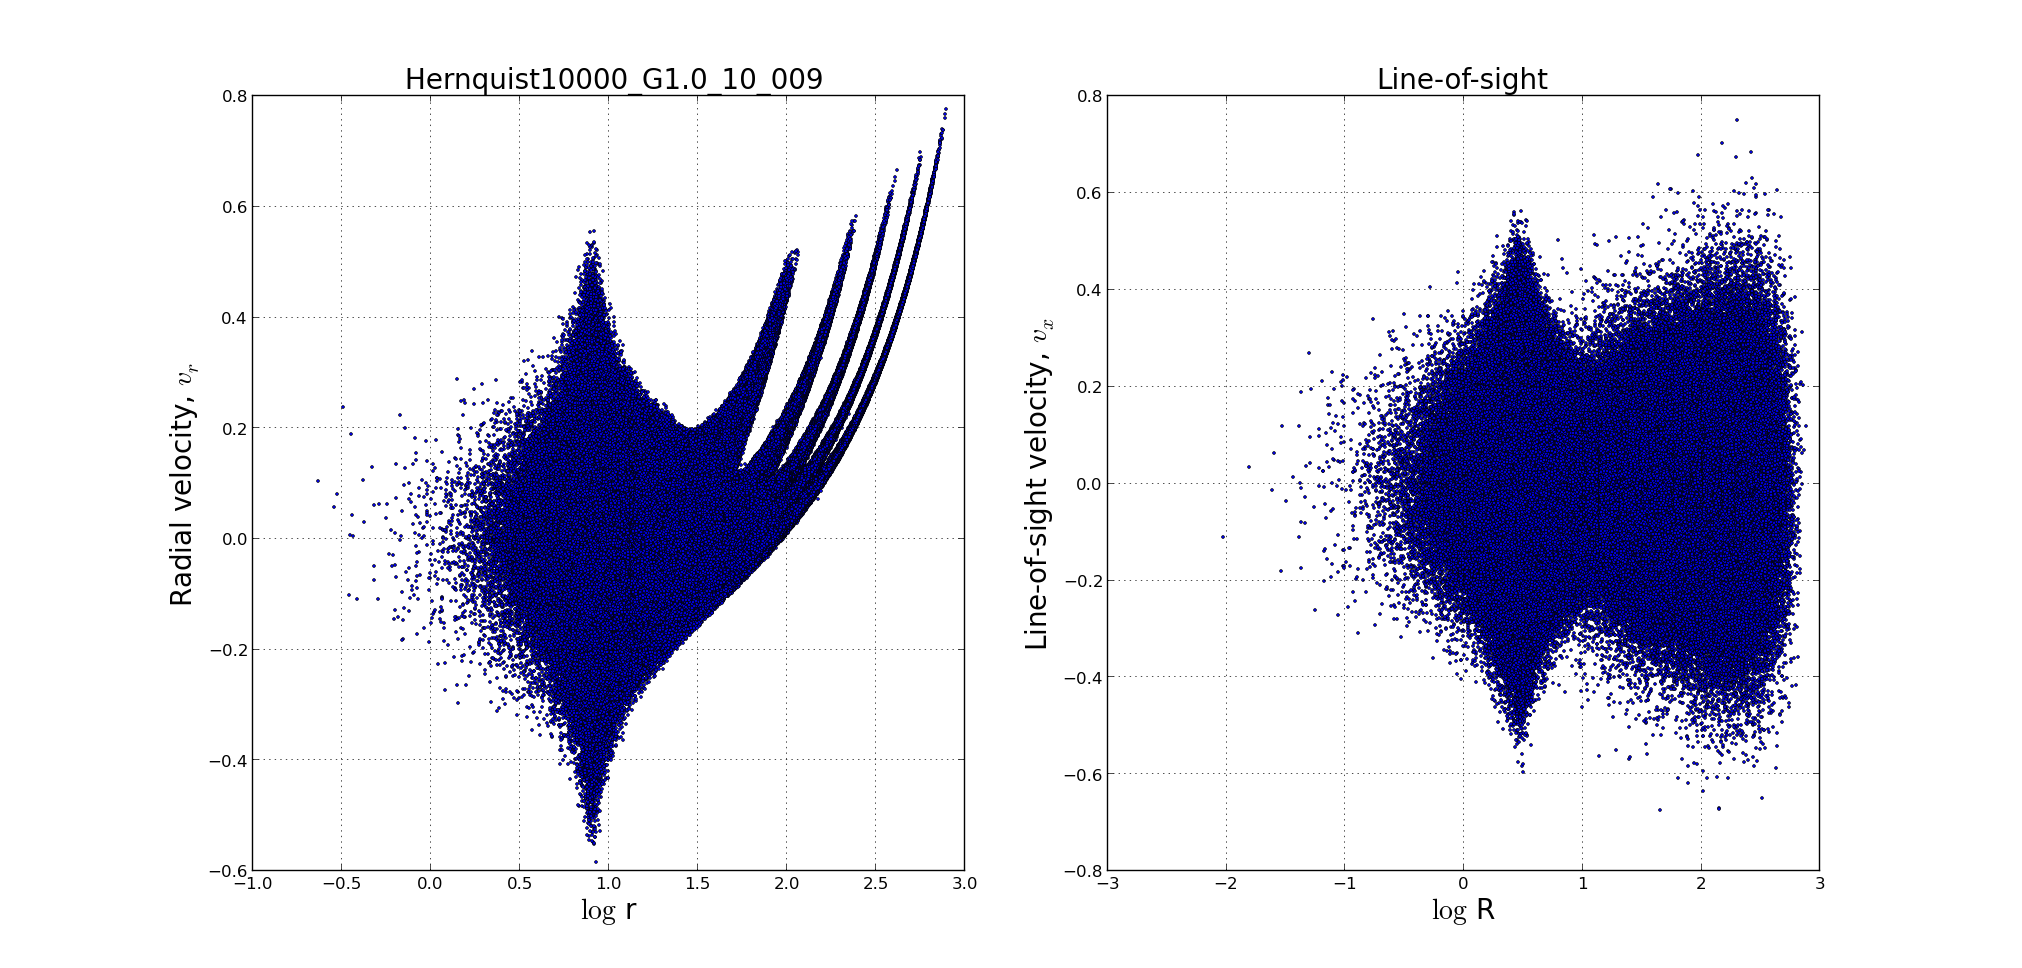
\includegraphics[width=1.0\linewidth]{img/LOS_logr.png}
\caption{For the file Hernquist10000$\_$G1.0$\_$10$\_$009 containing $10^6$ particles we here see a comparison of the radial velocity as function of logarithmic radius (left panel) to the LOS-velocity vs the logarithmic projected radius. This gives a great resolution of the center.}
\label{fig:test}
\end{figure}

\begin{figure}
\centering
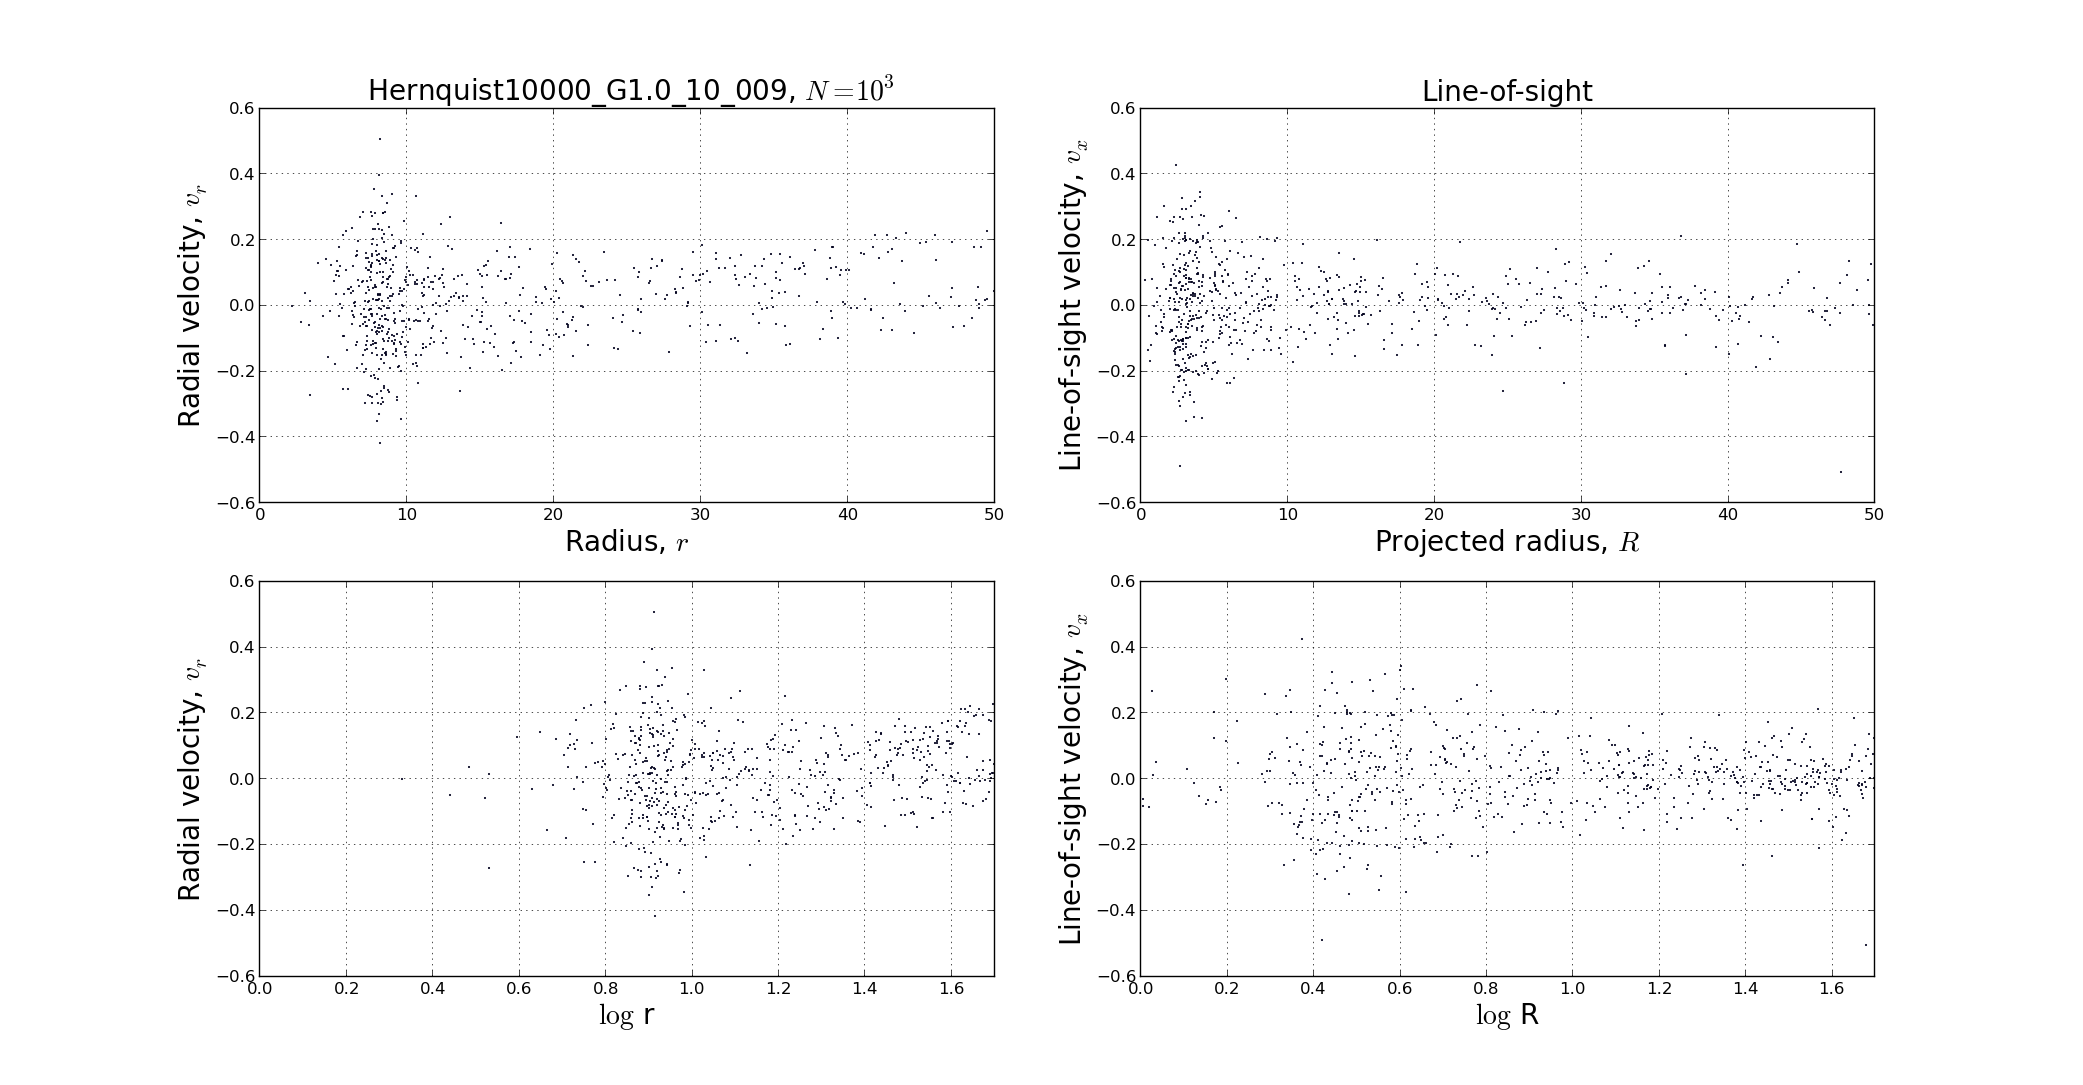
\includegraphics[width=1.0\linewidth]{img/LOS_radius50_N1000.png}
\caption{For the file Hernquist10000$\_$G1.0$\_$10$\_$009 we here see a comparison of the radial velocity as function of radius and logarithmic radius (left panel) to the LOS-velocity vs the projected radius and logarithmic projected radius. A thousand particles have been picked out for this analysis and the structure is cut off at radius = 50.
Looking at the top left subplot, basically the same number of particles seems to be present both above and below the zero-line at inner and middle-regions. at $r>40$ positive radial velocities starts to dominate over negative ones indicating a small particle flow away from the structure at large radii. This is expected as outer particles are less bound and might not have had sufficient time to reach equilibrium.}
\label{fig:test}
\end{figure}

This figure shows the inner part (up to radius 50) of the phase-space volume for particles in the file Hernquist10000$\_$G1.0$\_$10$\_$009.
If we pay close attention to the zero-line on the y-axis, in general we find as many particles over as under this line in the most central part up until about radius 20.
The central part is thus symmetric around the zero line. At higher radii there tend to be more particles with positive radial velocities which are the ones that has escaped the structure and will continue heading outwards forever.
This means that the central phase-space volume of particles are in equilibrium, but the outer part is not. The outer particles below the horizontal zero-line are heading towards the central phase-space volume again. This is particles experiencing a bit of infall.  We can thus track the particles which are no longer bound.

\newpage
\subsection{The bumpy road to universalities}

\begin{figure}
\centering
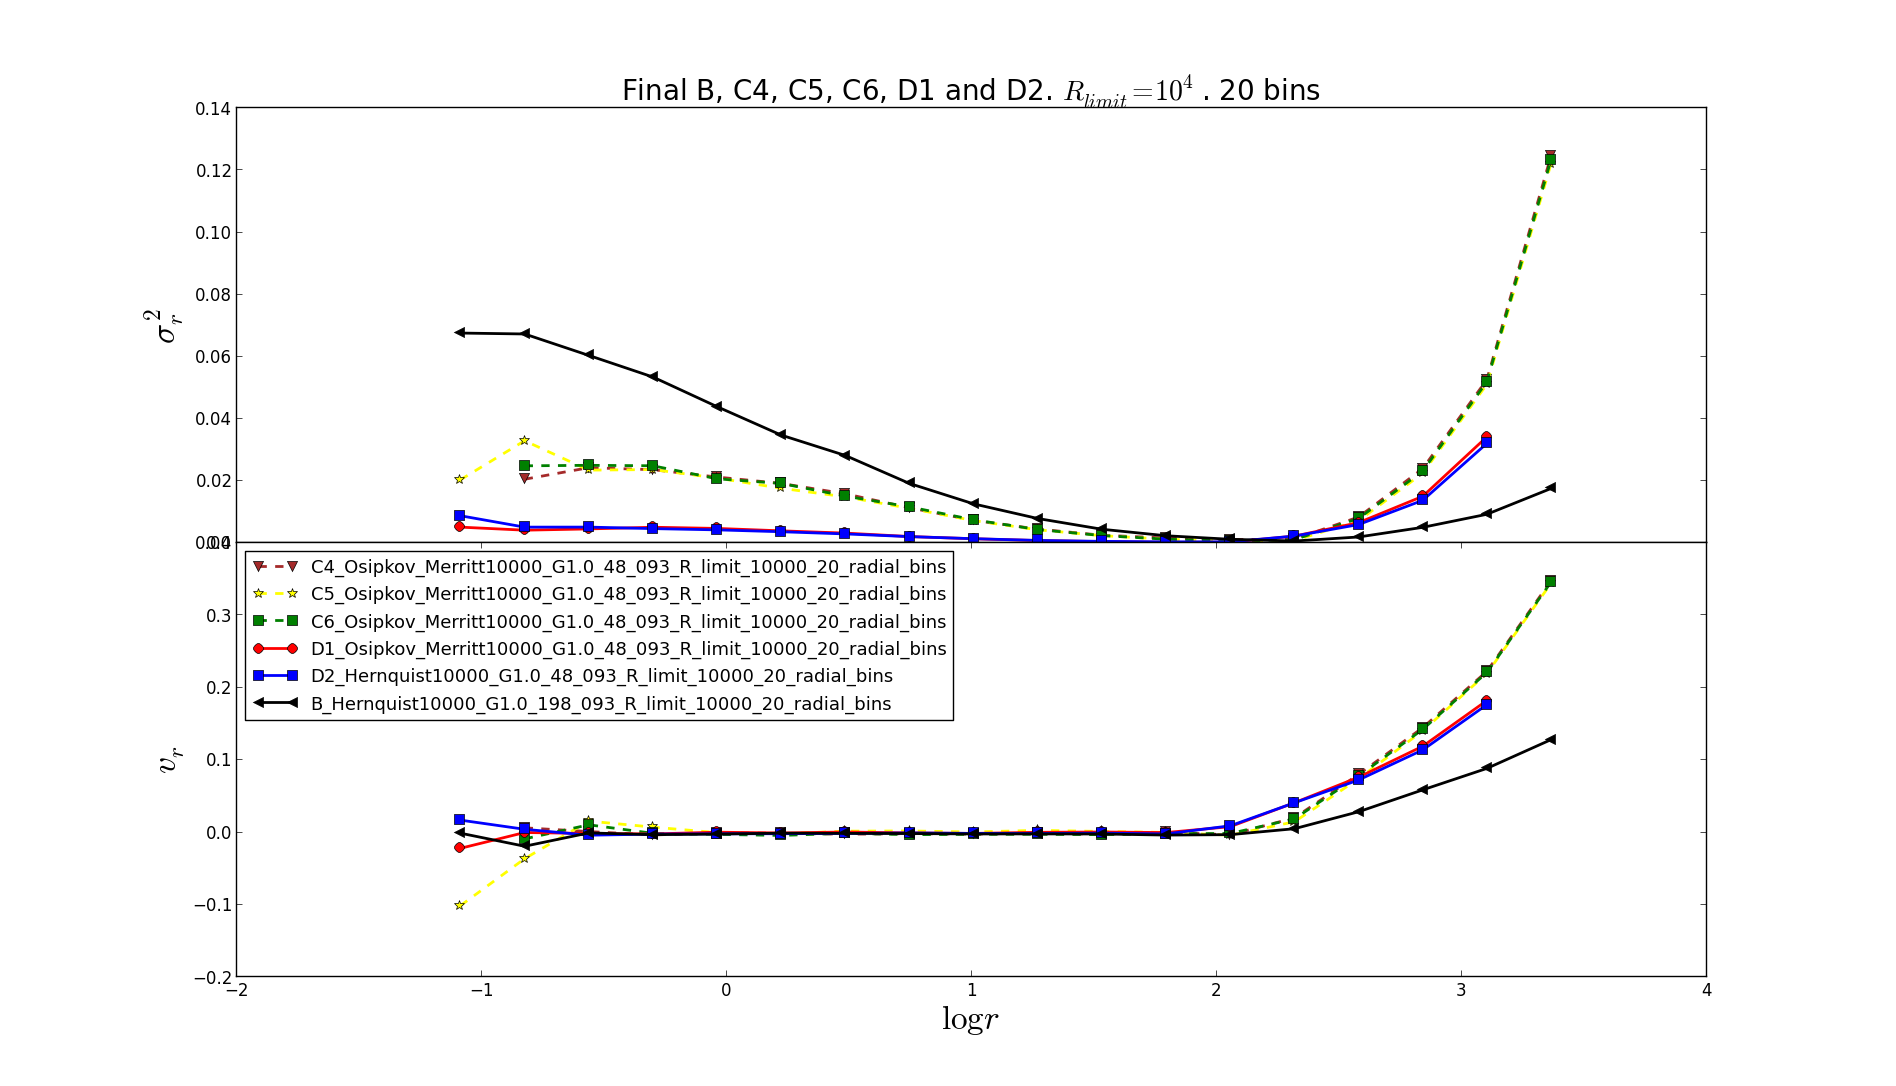
\includegraphics[width=1.0\linewidth]{img/BC4C5C6D1D2_sigmar2_vr_logr_panel.png}
\caption{The final products for the simulations \emph{B, $C_4$, $C_5$, $C_6$, $D_1$ and $D_2$}. Here $\sigma_r^2$ vs. logarithmic radius and radial velocity vs the logarithmic radius is shown. $N = 10^5$ particles are used for this analysis and the structure is cut off at radius = 10000.}
\label{fig:test}
\end{figure}

From the top panel of figure 51 there appear to be some overall trends to $\sigma_r^2$:
in the inner part, Sim B clearly has the largest $\sigma_r^2$, which then becomes smaller than the other simulations $\sigma_r^2$ in the outer part. 
From the bottom panel of figure 51 it is seen that on average there is the same amount of radial velocities above and below the zero line at inner and middle regions. This indicates the structures are in equilibria here and their particles are gravitationally bound. The outer region has an increase in radial velocities due to a few unbound particles which dominate the picture here. These have later been removed from the structures which then become flattened in this type of plot even for outer regions.

\begin{figure}
\centering
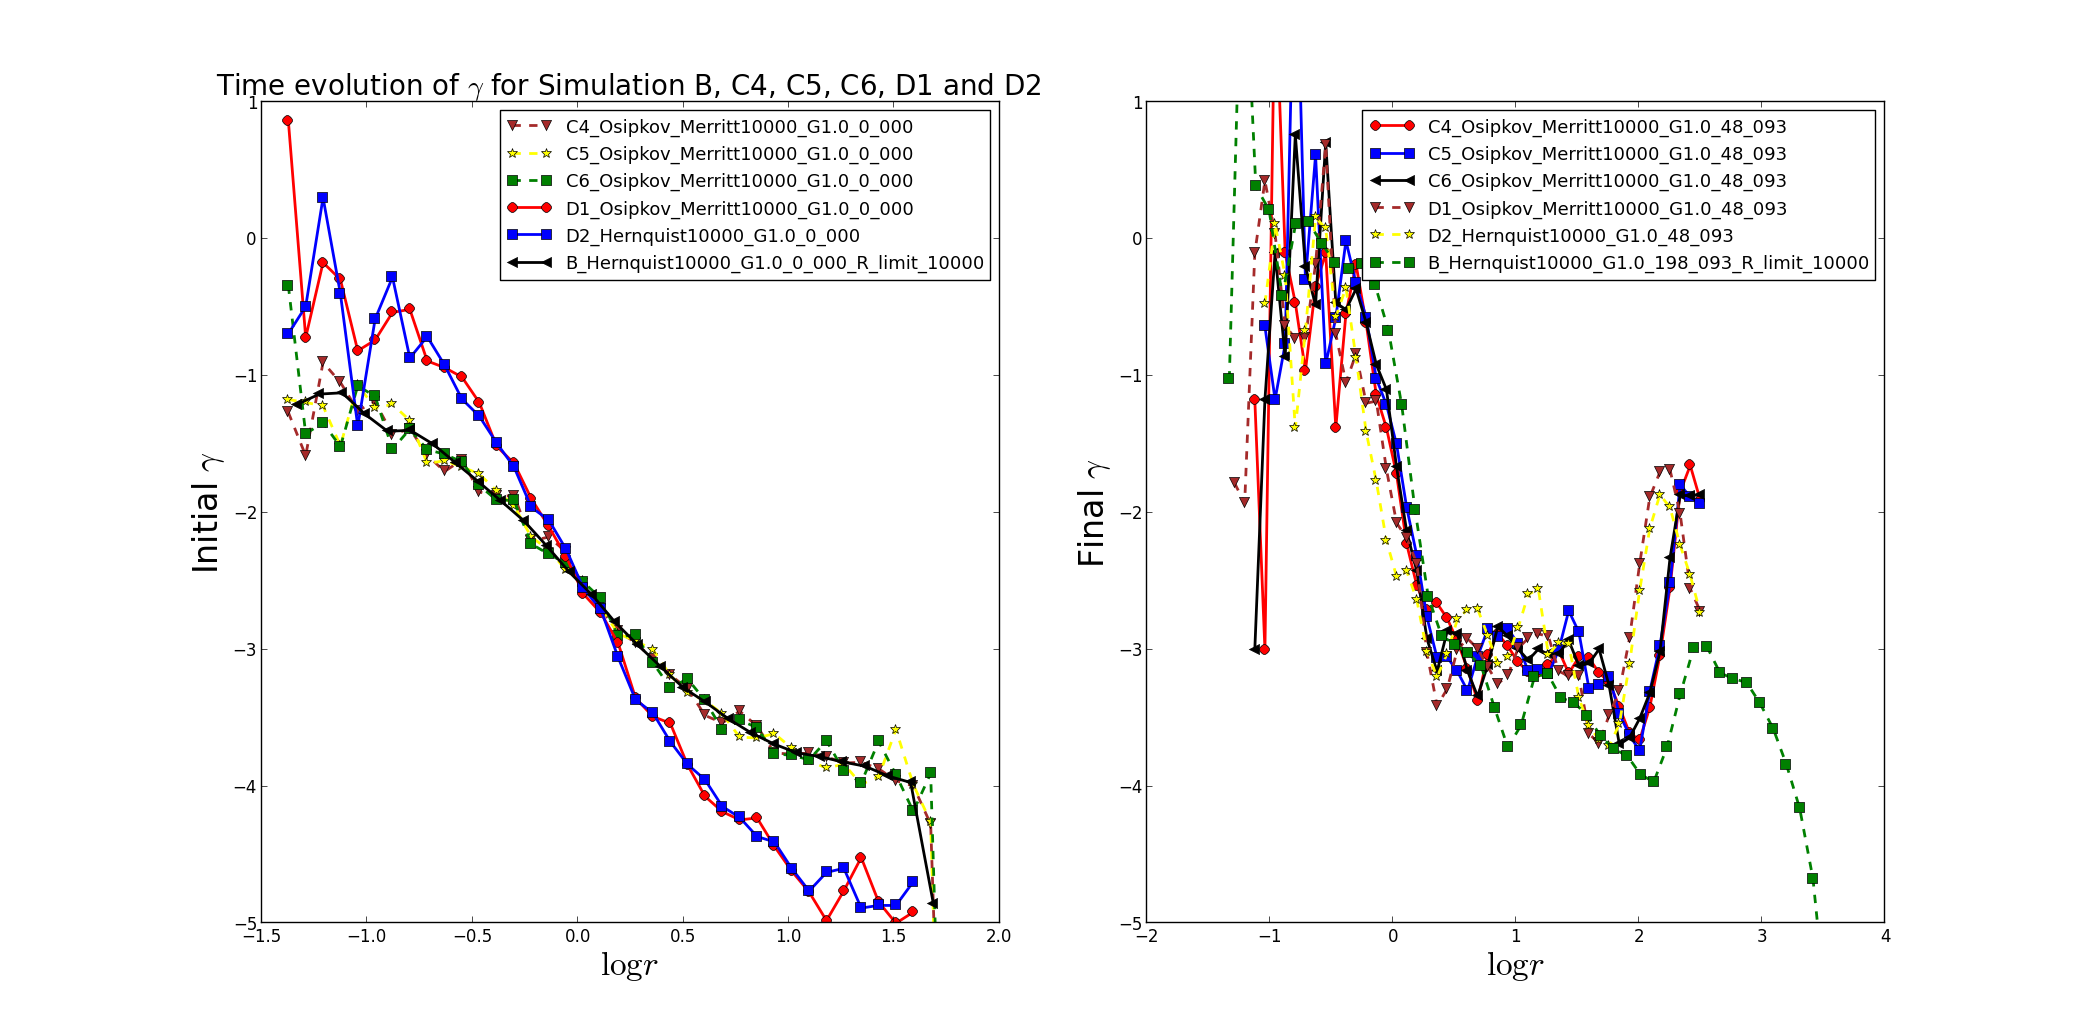
\includegraphics[width=1.0\linewidth]{img/BC4C5C6D1D2_gamma.png}
\caption{IC and final products for the simulations \emph{B, $C_4$, $C_5$, $C_6$, $D_1$ and $D_2$}.
The final products show universal trends: there seem to be three distinct local minima and similarly three distinct local maxima to the $\gamma$ profiles at the outer volume (where $\log r > 1 $) of the various structures. For $D_1$ and $D_2$ the extrema almost overlap, which is also the case for $C_4$, $C_5$ and $C_6$. B has unique positions of extrema.}
\label{fig:test}
\end{figure}

\begin{figure}
\centering
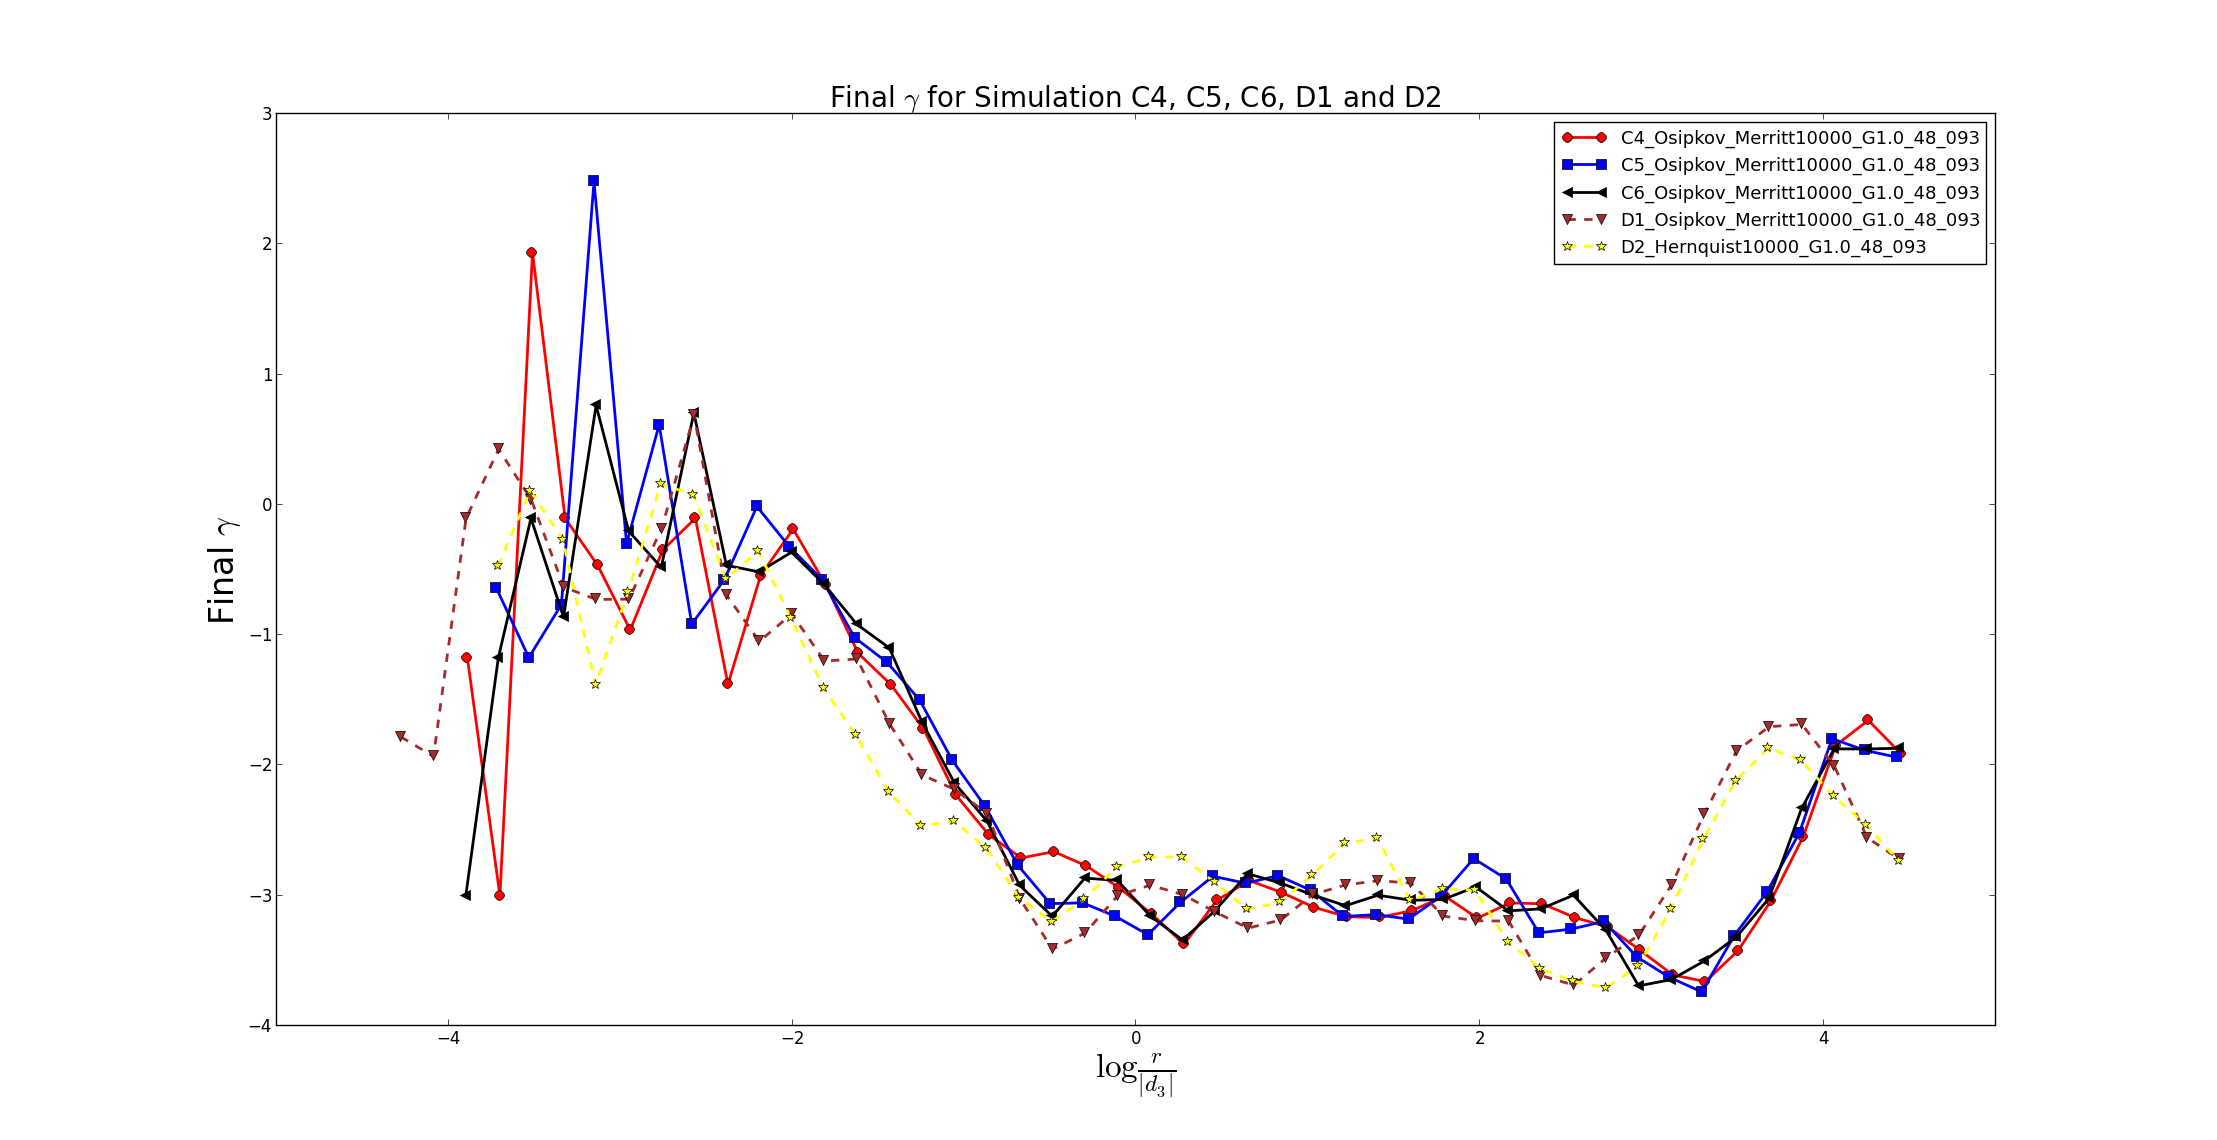
\includegraphics[width=1.0\linewidth]{img/C4C5C6D1D2_gamma_d3.png}
\caption{Final products for the simulations \emph{$C_4$, $C_5$, $C_6$, $D_1$ and $D_2$}.
Here the individual $\gamma$ profiles are shown vs. $\log ( \frac{r}{d_3})$, where $d_3$ are the $\gamma$-value of each profile at its third local minima. }
\label{fig:test}
\end{figure}

\begin{figure}
\centering
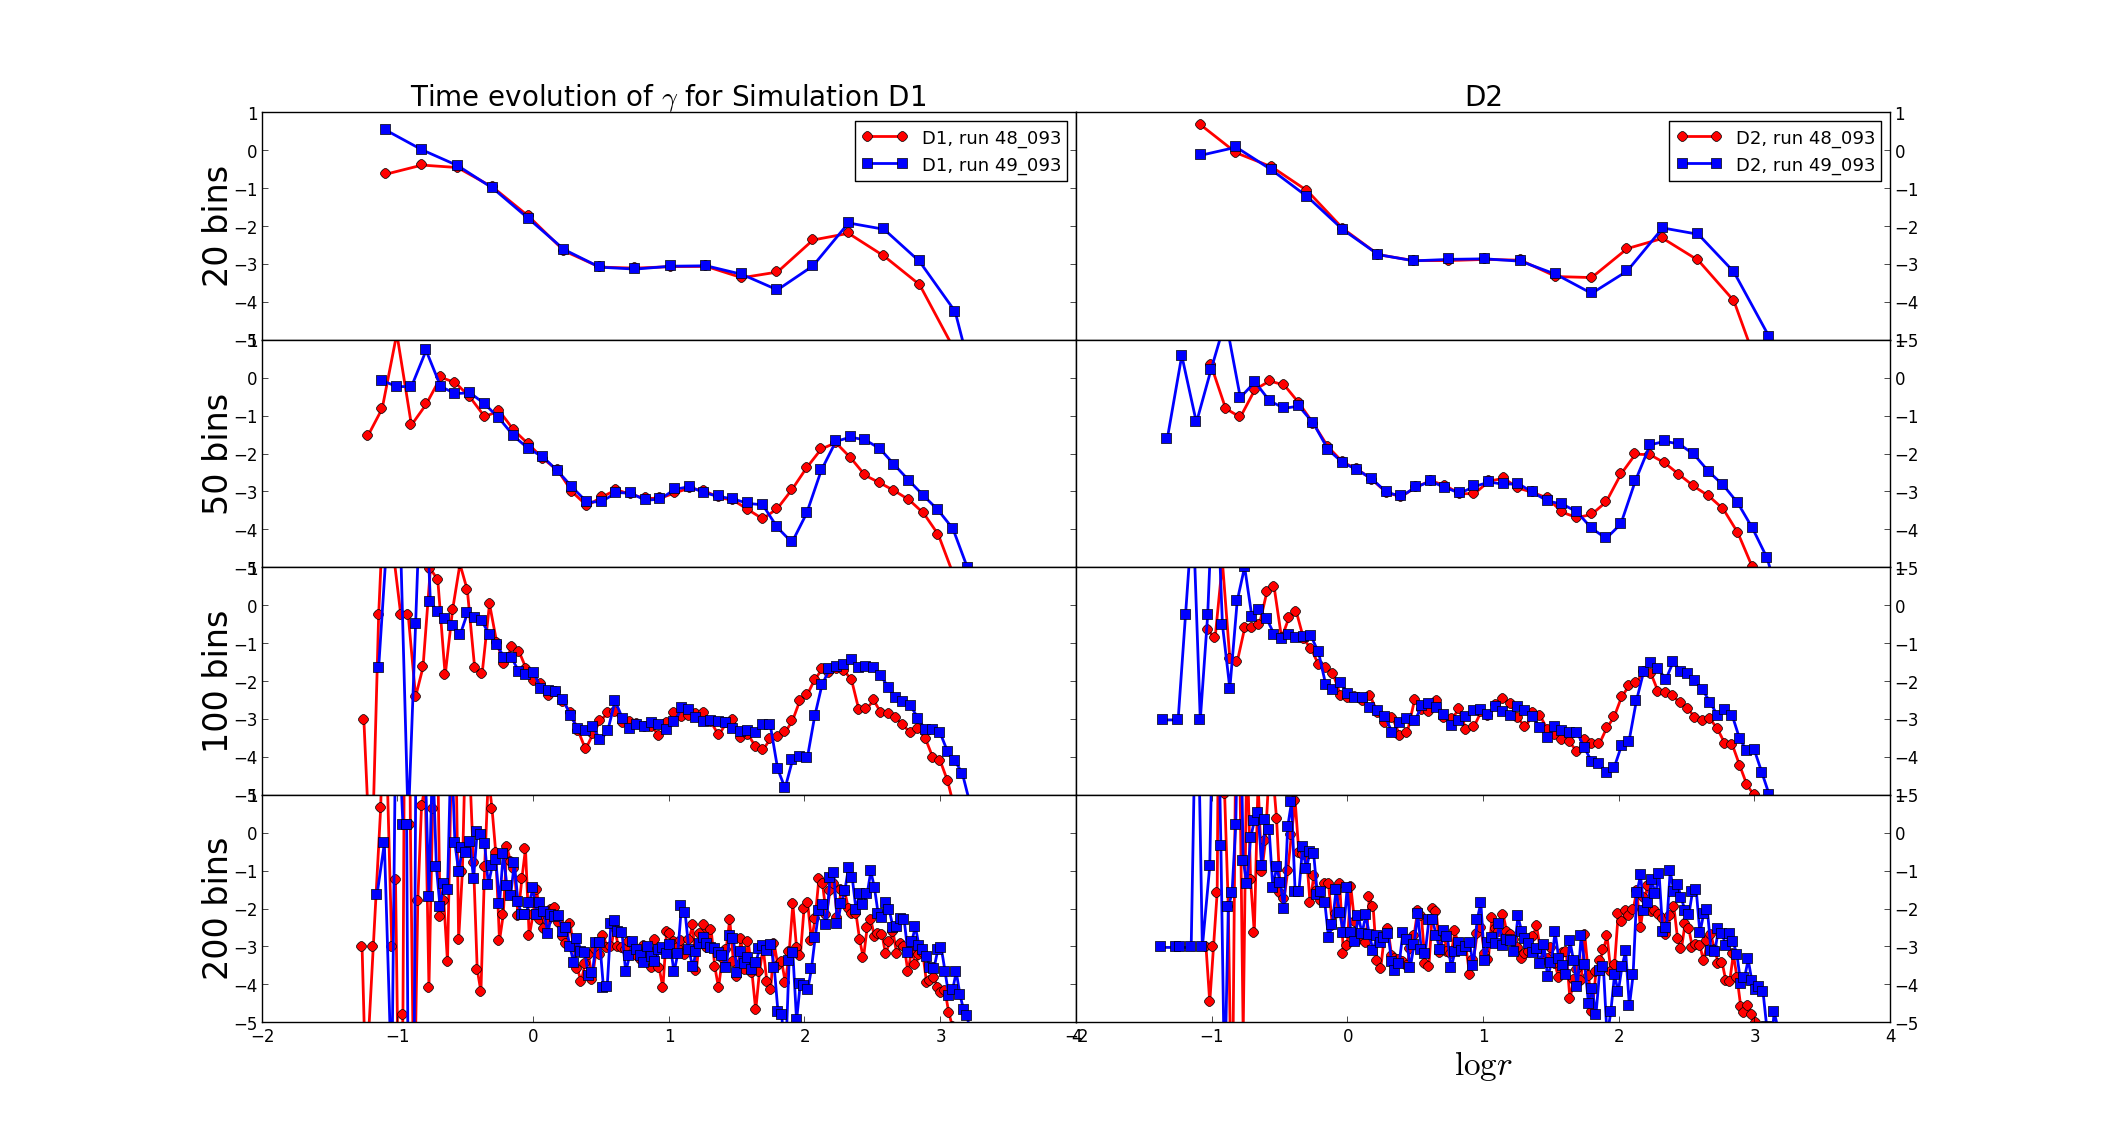
\includegraphics[width=1.0\linewidth]{img/D1D2_gamma_logr_panel.png}
\caption{Time evolution of $\gamma$-profile for the final states of the unstable structure $D_1$ (left panel) and the final states of the stable structure $D_2$ (right panel) from sim. I. From the top and downwards the number of radial bins is 20, 50, 100 and 200 respectively. The final states are 48$\_$093
and 49$\_$093 for both structures. From plots like these it is concluded that the optimum number of radial bins for structures with $N = 10^5$ particles is 20 and that the optimum number of radial bins for structures with $N = 10^6$ particles is 50.}
\label{fig:test}
\end{figure}

\begin{figure}
\centering
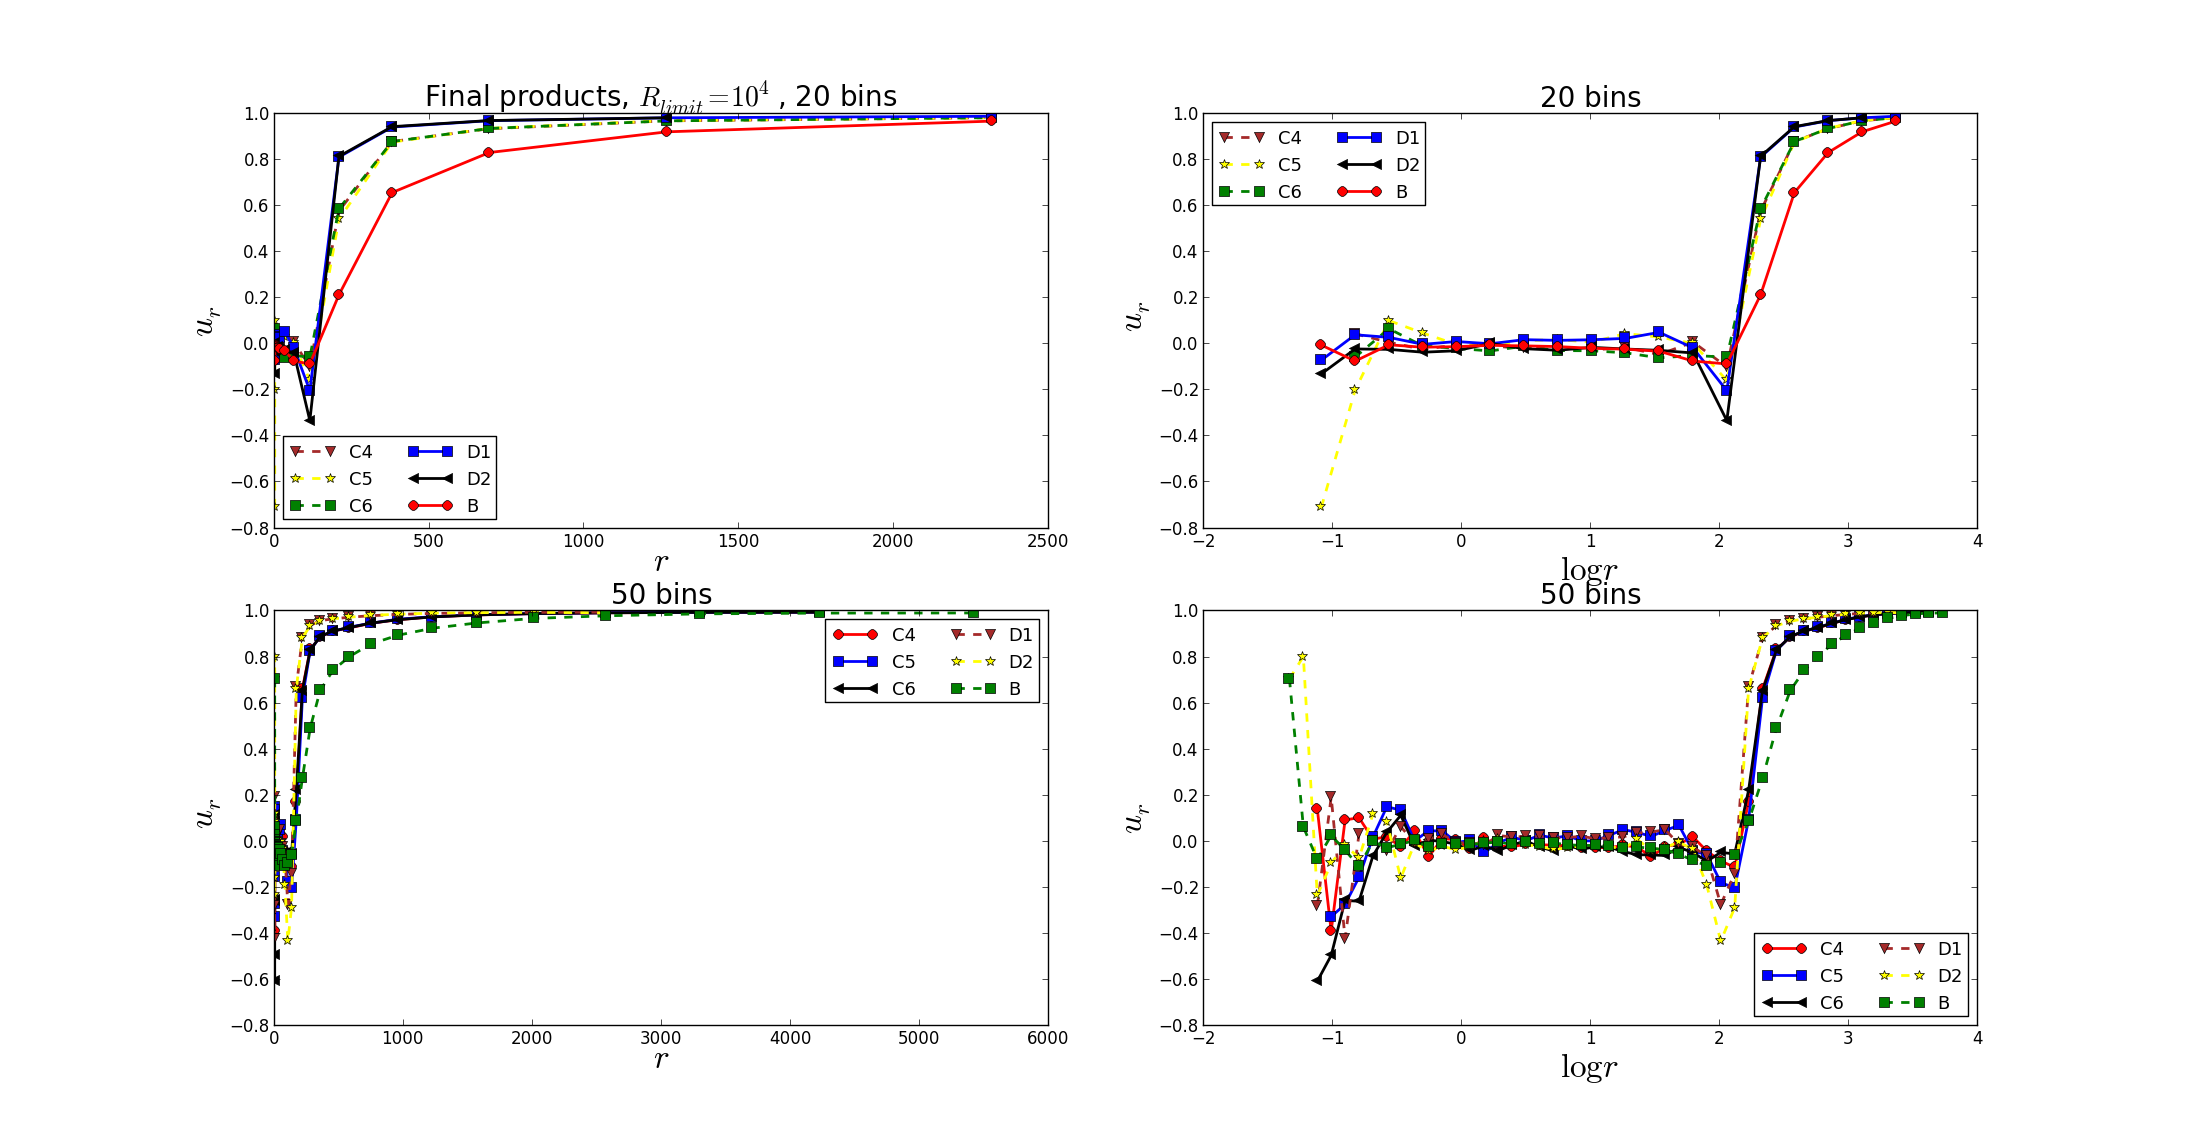
\includegraphics[width=1.0\linewidth]{img/BC4C5C6D1D2_r_logr_ur_mean_timemax_4600.png}
\caption{Final products for the simulations \emph{B, $C_4$, $C_5$, $C_6$, $D_1$ and $D_2$}.
Here the radial velocities divided by the radial velocity dispersions are shown vs. r and $\log r $, for both 50 and 20 radial bins. }
\label{fig:test}
\end{figure}

\begin{figure}
\centering
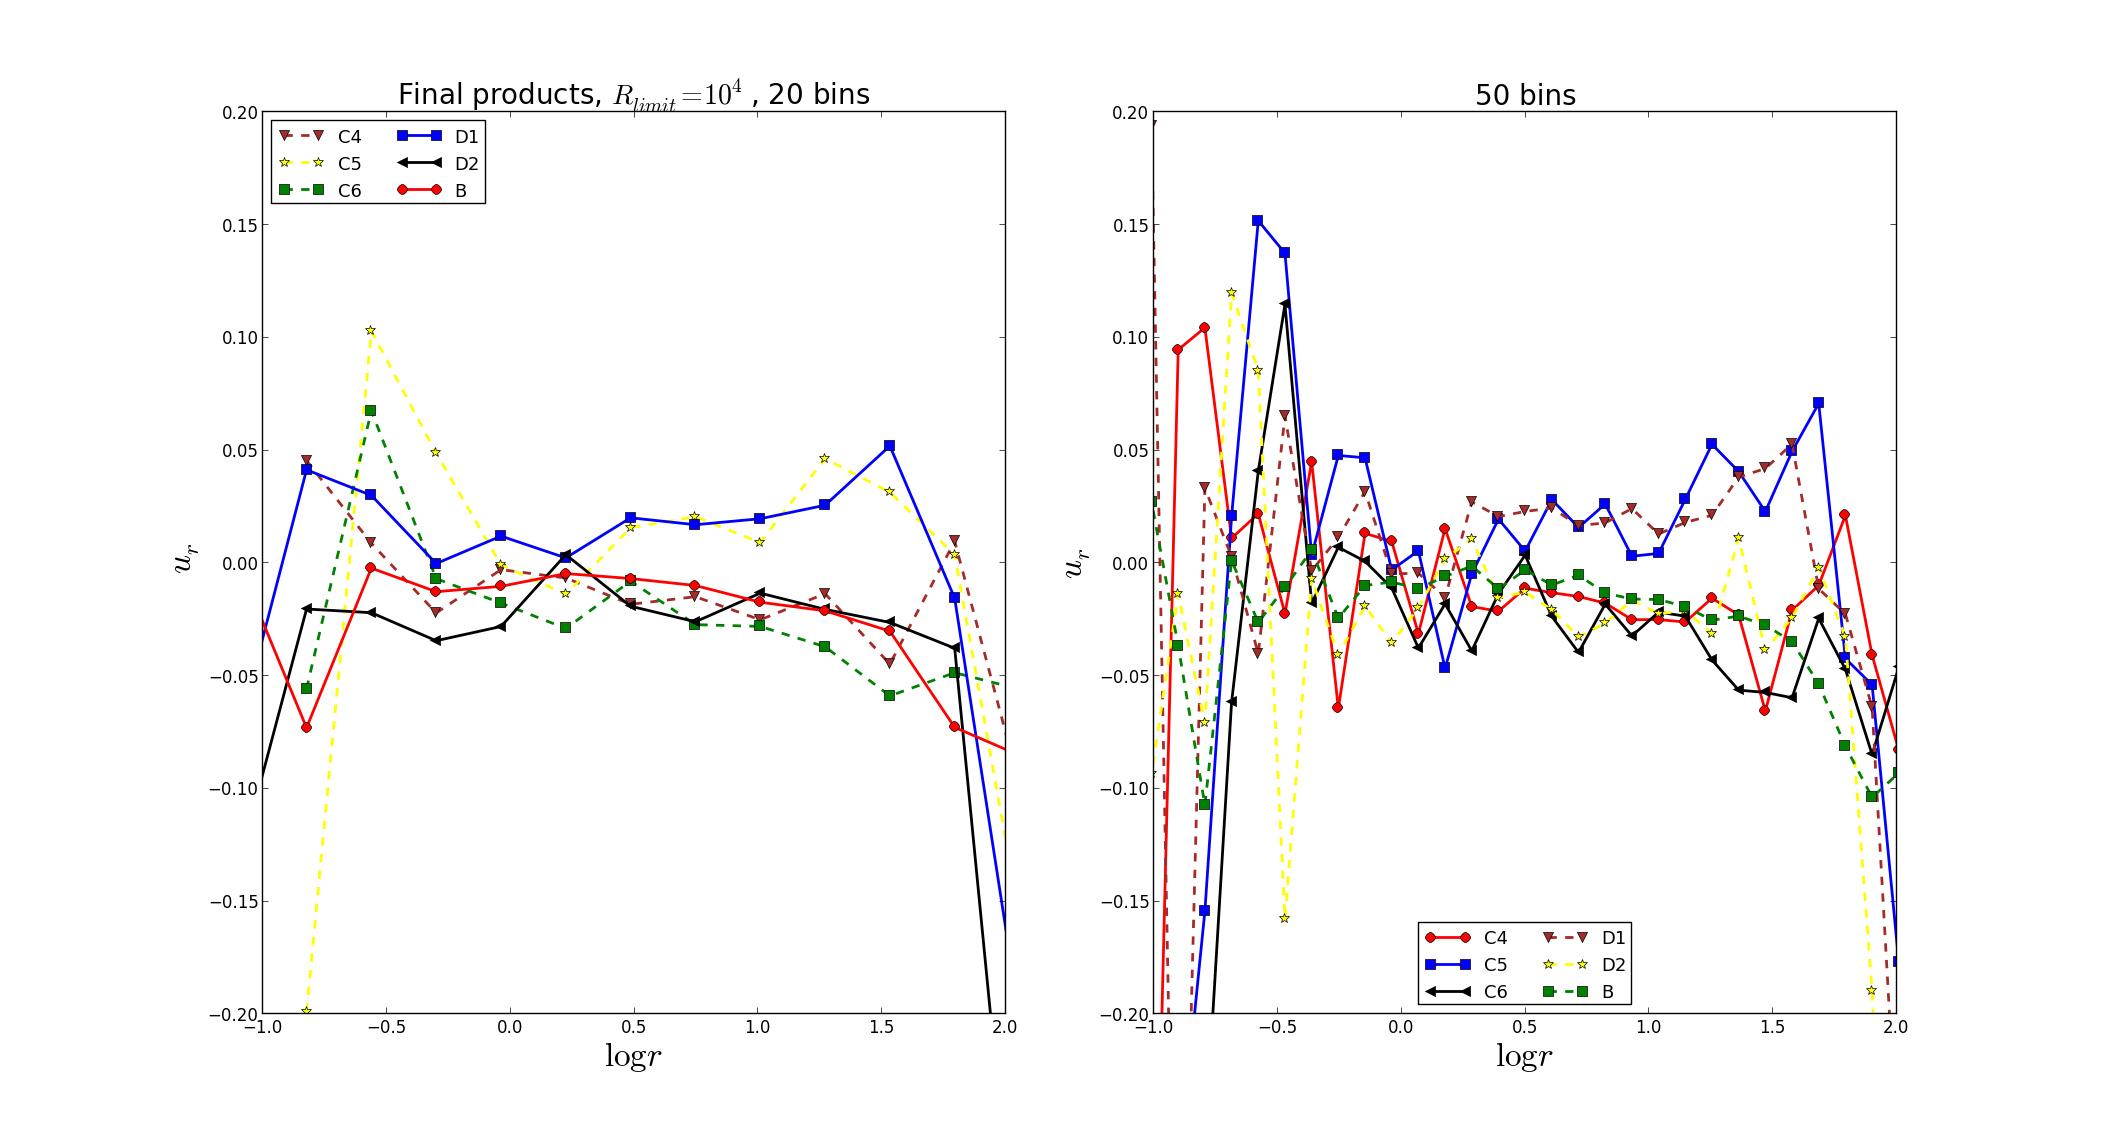
\includegraphics[width=1.0\linewidth]{img/BC4C5C6D1D2_logr_ur_mean_timemax_4600_zoom.png}
\caption{Zoom in on previous figure. Due to Poisson noise, the regions logr < -1 and logr > 2 can not be trusted. The vertical axis showing $u_r$ has also been narrowed down to a smaller range for more clarity.}
\label{fig:test}
\end{figure}